\documentclass{article}

\usepackage{graphicx}
\usepackage{wrapfig}
\usepackage{pgfplots}
\usepackage[oldvoltagedirection]{circuitikz}
\usepackage{titling}

\usepackage{fancyhdr}
\usepackage{mathtools}
\usepackage{scalerel}
\usepackage{amssymb}
\usepackage{stackengine}
\usepackage[parfill]{parskip}
\usepackage[margin=1in]{geometry}
\usepackage[makeroom]{cancel}
\pgfplotsset{compat=1.16}

\everymath{\displaystyle}
\graphicspath{{../}}
\usepgfplotslibrary{fillbetween}
\date{2\textsuperscript{o} Semestre 2018/19}
\title{Sistemi di Telecomunicazione}
\author{ale-cci }

\renewcommand\maketitlehooka{\null\mbox{}\vfill}
\renewcommand\maketitlehookd{\vfill\null}

\pagestyle{fancy}

\def\myupbracefill#1{\rotatebox{90}{\stretchto{\{}{#1}}}
\def\rlwd{.5pt}
\newcommand\notate[4][B]{%
  \if B#1\else\def\myupbracefill##1{}\fi%
  \def\useanchorwidth{T}%
  \setbox0=\hbox{$\displaystyle#2$}%
  \def\stackalignment{c}\stackunder[-6pt]{%
    \def\stackalignment{c}\stackunder[-1.5pt]{%
      \stackunder[2pt]{\strut $\displaystyle#2$}{\myupbracefill{\wd0}}}{%
    \rule{\rlwd}{#3\baselineskip}}}{%
  \strut\kern9pt$\rightarrow$\smash{\rlap{$~\displaystyle#4$}}}%
}

\DeclareMathOperator*{\argmax}{argmax}
\DeclareMathOperator*{\argmin}{argmin}
\DeclareMathOperator\erf{erf}
\DeclareMathOperator\snr{SNR}
\DeclareMathOperator\erfc{erfc}


\begin{document}
\begin{titlingpage}
\maketitle
\end{titlingpage}
\newpage

\tableofcontents

\newpage
%% -- Begin --

\section{Guadagno in potenza}

\[
    P_{out} = gP_{in}  \xrightarrow[]{10\log_{10}{}} P_{out_{db}} = g_{db} + P_{in_{db}}
\]

\begin{itemize}
    \item $g < 1$: Perdita di Trasmisione

    \item $L$: Transmission Loss $\coloneqq \quad g^{-1}=\frac{P_{in}}{P_{out}}$

\end{itemize}

\subsection{Attenuazione di tipo Radio}
Sistemi di telecomunicazione su cao (Dal nome, Segnale si propaga lungo un cavo)

\begin{itemize}
    \item $l$: lunghezza del cavo
    \item $\alpha$: coefficente d'attenuazione $\frac{dB}{Km}$
\end{itemize}

\[
    \notate{P_{out}}{2}{\text{Da fisica}} = \notate{10^{-\frac{\alpha}{10}l} P_{in} }{1}{\text{$\cdot < 1 $ Siccome $\alpha$ e $l$ sono positivi}}
\]

$g = 10^{+\frac{\alpha}{10}l}$

$L=10^{-\frac{\alpha}{10} l}$

$L_{dB} = 10\log_{10} L = \alpha \cdot l$


\begin{center}
    \begin{tabular}{||c|c|c||}
        \hline
        Esempi & Frequenza & \( \alpha \)     \\
        \hline \hline
        Doppino Telefonico & \( 10 kHz \) & 2 \\
                           & \( 100 kHz\) & 3 \\
                           & \( 300 kHz\) & 6 \\
        \hline
        Cavo Coassiale     & \( 100 kHz\) & 1 \\
                           & \( 1 MHz\) & 2 \\
                           & \( 3 MHz\) & 4 \\
        \hline
        Guida d'onda rettangolare     & \( 10 GHz\) & 5 \\

        \hline
        Cavo in fibra Ottica & \( 4\cdot 10^{14} Hz\) & 10 \\

        \hline
    \end{tabular}
\end{center}

Per ``combattere'' l'attenuazione vengono usati i ripetitori

\textbf{Trasmissione Radio}: Perdita di potenza dovuta all'irradiazione stessa

\begin{itemize}
    \item $l$: distanza
    \item $\lambda$: Lunghezza d'onda
    \item $\alpha$: path loss exponent
\end{itemize}


$ L = {(\frac{4\pi l}{\lambda})}^2 $


\framebox{$ C = \lambda f_c $} \quad
$f_c$ frequenza portante

$ L = {(\frac{4\pi l}{\lambda})}^\alpha $

$f_c$ \'e solamente espressa in $GHz$, quindi si ha che:

\[
    L_{dB} = 20\log_{10} {\left(\frac{4\pi}{\lambda}l\right)}^2 + 20\log_{10} 10^9 + 20\log_{10} f_{c_{GHz}} = 92.4 + 20\log_{10} l + 20\log_{10} f_{c_{GHz}}
\]

\subsection{Tramissioni Cablate}
$L_{dB} = \alpha l$

\textbf{Antenna Radio}: Soino dette \textbf{direttive}, se concentrano la potenza su un unica direzione

Piu l'antenna \'e direttiva, pi\'u \'e alto il guadagno

\underline{Esercizio}

\subsection{Formule di Friis}

\[
    P_{out} = P_{in} \frac{g_T g_R}{{(\frac{4 \pi d f_c} {C})}^\nu} \quad \rightarrow  \quad K{\left(\frac{1}{d}\right)}^\nu
\]

% diagram

\begin{itemize}
    \item \textbf{Shadowing}: Fluttuazione dovuta a cambiamento dell'ambiente
    \item \textbf{Short Term Fading}: Fluttuazione a breve distanza, distribuita come la \textit{distribuzione di Reileigh}
\end{itemize}

\subsection{Dominio Frequenziale}

$S_y(f) =S_x(f) {\lvert H(f) \rvert}^2$

% grafico 1 %
% grafico 2 %
$B_c$: Banda di Coerenza $\rightarrow$
Intervallo frequenziale in cui la risposta  in frequenza del canale varia di poco

$B_c > B$: Canale \textbf{NON} selettio di frequenza, La risposta del canale ``non'' cambia su $T_s$ (Tempo di fading) lento ($T_s < T_c$)


$B_c < B$: Canale Selettivo in frequenza
fading veloce: risposta cambia su $T_s$ $(T_s > T_c)$

% immagine antenne %

$B_c = \frac{1}{5\sigma_D}$

$T_s$: Tempo di simbolo

$T_c = \frac{6}{16\pi f_D}$

$f_D$: Frequenza Doppler

\newpage
\section{Modello ISO-OSI}

\begin{enumerate}
    \item Phisical
    \item Data-Link
    \item Network
    \item Transport
    \item Session
    \item Presentation
    \item Application
\end{enumerate}

\textbf{Tabelle di Routing} Protocollo IP Riesce a trovare il percorso tra utente ed endpoint

\subsection{Livello 1}
perso

% image %

\subsection{Livello 2}
Trasmette i grame al nodo successivo
\begin{itemize}
    \item Controlla che il lin sia attivo
    \item Fornisce informazione ai livelli superiori
    \item Correzione errore per frame
\end{itemize}

\textbf{MAC}: Medium Access Control

\textbf{LLC}: Logical Link Control $\rightarrow$ controlla che il link sia attivo


\subsection{Livello 3}
Si occupa solo del \textbf{percorso logico} tra due punti, non compe vengono trasferiti i dati

Nasconde i livelli inferiiori ai layer superiori rendendoli hardware-independent

\subsection{Livello 4}
Consegna messaggio tra due processi
% dual split

\subsection{Livello 5}
Abilita, Modifica, Termina sessioni tra applicazioni

Pi\'u connessioni possono essere viste come una singola sessione

Distingue i dati che arrivano tra ``application data'' (dati usati dalle applicazioni) e ``session control data''.

Usa dati dei layer 3\&4 per monitorare la comunicazione tra applicazioni

Translation for naming services (google.com $\rightarrow$ 8.8.4.4)

\subsection{Livello 6}
Translation, Compression, Decription and Encapsulation of Data, (Es: Html, JPG, Ascii\ldots)

\subsection{Livello 7}
Fornisce servizi di comunicazione alle applicazioni, esempi ne sono: Http e FTP

\section{TCP/IP}
Inizialmente suddiviso in 4 layer:

\begin{itemize}
    \item Host to Network
    \item Internet
    \item Transport
    \item Application
\end{itemize}

Ma se confrontato al modello OSI ne si possono riconoscere 5:

\begin{itemize}
    \item Application
    \item Transport
    \item Network
    \item Data Link
    \item Phisical
\end{itemize}

In una rete TCP/IP vengono usati 4 livelli di indirizzi

\begin{itemize}
    \item Phisical
    \item Logical
    \item Port
    \item Application-Specific
\end{itemize}

\section{Struttura generale di un sistema di comunicazione}
% image

\textbf{Capacit\'a di canale ($C$)}: Massima velocit\'a a cui possono essere trasmessi i dati

\textbf{Data rate ($bps$)}: Dati effettvamente comunicati

\textbf{BandWidth ($B$)}: la grandezza di banda del segnale trasmesso

\textbf{Bit Error Rate ($BER$)}: Frequenza con cui avvengono erriri di trasmissione

\section{Modulazione}
Aggiungere informazioni al segnale portante $x(t)$
\[
    x(t) = A\cos(2\pi ft + \Phi)
\]

$A$: Ampiezza

$f$: Frequenza

$\Phi$: Fase

Carrier signal: $x(t)$ su cui sono state modulate le informazioni
Analog to analog conversion: Needed only if a bandpass is available

\begin{samepage}
    \begin{itemize}
        \item Aplitude modulation
        \item Frequency modulation
        \item Phase modulation
    \end{itemize}
\end{samepage}

\subsection{Amplitude modulation (AM)}
\begin{itemize}
    \item $m(t)$: Information signal
    \item $A_c\cos(2 \pi f_c t)$: carrier
    \item $f_c$: Carrier frequency
\end{itemize}

Total Bandwidth: $2B$

\[S(t) = A_c(1 + K_o m(t)) \cos(2\pi f_c t)\]

\[\quad \Big\Downarrow \mathcal{F} \quad \]

\[S(f) = \frac{A_c}{2} \left[ \delta(f - f_c) + \delta(f+f_c) + K_o M(f - f_c) + K_o M(f+f_c)\right]\]

%immagine

\subsection{Frequency modulation FM}

\begin{minipage}[]{0.5\textwidth}
    \[
    S(t) = A_c \cos(\theta(t))
    \]
    % first image
\end{minipage}
\begin{minipage}[]{0.5\textwidth}
    \[
        m(t) \coloneqq \frac{ d\theta(t)}{dt} = 2\pi f_c + 2\pi K_f m(t)
    \]
    % second image
\end{minipage}

\textbf{$K_f$}: Frequency derivation constant $\frac{Hz}{V}$

\subsection{Phase Modulation PM}
\[
    S(t) = A_c \cos(2\pi f_c t + K_p m(t))
\]

La variazione di fase si manifesta come una variazione istantanea di frequenza, (proporzionale alla derivata di m)

\textit{Total Bandwidth}: $6B$

Le modulazioni lineari occupano meno banda $\rightarrow$ utilizzate per accomodare pi\'u utenti

Se l'informazione da trasmetter non \'e Analogica ma digitale, la modulazione si chiama Keying

\begin{minipage}[t]{0.5\textwidth}
    \textbf{Amplitude shift Keying ASK}
    \begin{itemize}
        \item $f$ \'e costante
        \item low bandwidth
        \item weak against interference
    \end{itemize}
\end{minipage}
\begin{minipage}[t]{0.5\textwidth}
    \textbf{Frequency shift Keying FSK}

    \[
        FSK(t) =
        \begin{cases*}
            \sin(2\pi f_1 t) \\
            \sin(2\pi f_2 t)
        \end{cases*}
    \]

    % image
    \begin{itemize}
        \item More bandwidth required
    \end{itemize}
\end{minipage}

\subsection{Phase Shift Keying (PSK)}
\[
    \text{PSK}(t) =
    \begin{cases}
        \sin (2\pi f t)\\
        \sin (2 \pi f t + \pi)
    \end{cases}
\]
\begin{itemize}
    \item More complex
    \item Strong against interference
\end{itemize}

\subsection{Binary Phase Shift Keying (BPSK)}
\[
    \text{BPSK}(t) =
    \begin{cases}
        \sqrt{\frac{2E_b}{T_b}} \cos (2\pi f_c t + \delta_c)\\
        \sqrt{\frac{2E_b}{T_b}} \cos (2\pi f_c t + \pi \delta_c)
    \end{cases}
    \qquad \text{con} \quad 0 < t < T_b
\]
\begin{itemize}
    \item $T_b$ Tempo di Bit
    \item $E_b$ Energia di Bit
\end{itemize}

\subsection{Quadrature Phase Shift Keying (QPSK)}
La fase della portante assume 5 valori separati di $\frac{\pi}{2}$. Ogni fase corrisponde ad una coppia unica di bit

\[
    S_{\text{QPSK}}(t) = \sqrt{{2E_b}{T_b}} \cos (2\pi f_c t + i\frac{\pi}{2}) \qquad \text{con} \quad i \in 0..3
\]

La larghezza di banda \'e la met\'a della BPSK

Pu\'o essere espressa come 2 BPSK, il bit-error-rate rimane lo stesso ma la Banda utiilzzata raddoppia

(X: Diagramma a costellazione)

\subsection{Multi-? Phase and Amplitude modulation}
(X: 16Qam, 16psk 16apsk )
Pi\'u i punti sono vicini, pi\'u sono sensibili al rumore

\subsection{Capacit\'a di Canale AWGN (Additive White Gaussian Noise)}
\begin{minipage}{0.4\textwidth}
\[
    C = B\log_2(1 + \frac{P_{in}}{P_{out}})
\]
\[ P_N = B \dot N_0 \qquad \rho \coloneqq \frac{R}{B} \]
\[
    \begin{cases}
        C = B\log_2\left( 1 + \frac{P_{in}}{BN_0}\right)\\
        R \le C
    \end{cases}
\]
\[  \frac{R}{B} \le \log_2\left(1 + \frac{E_b \cdot R}{N_0B}\right) \]
\[  \frac{R}{B} \le \log_2\left(1 + \frac{R}{B}\gamma_b\right) \]
\[ \rho \le \log_2 \left( 1 + \rho \gamma_b\right) \]

\framebox{\textbf{Rumore Bianco} \( \sim \mathcal{N}(0, \sigma^2) \rightarrow n(t) = \frac{1}{\sqrt{2\pi\sigma^2}} e^{-\frac{t^2}{2\sigma^2}} \)}
\end{minipage}
\begin{minipage}{0.6\textwidth}
    \begin{itemize}
        \item $P_{in}$: Potenza Segnale in ingresso
        \item $B$: Banda del Canale
        \item $P_N$: Potenza del Rumore Bianco (Gaussiano)
        \item $N_0$ Densit\'a spettrale di potenza del rumore
        \item $\rho$: Efficenza Spettrale
        \item $R$: Data Rate Utilizzato
        \item $\gamma_b$: Signal Noise ratio $\coloneqq \frac{E_b}{N_0}$
    \end{itemize}
\end{minipage}

\subsection{Calcolo Errore su BPSK}
Ricordando che, da definizione:
\[ \erf(x) = \frac{2}{\sqrt{\pi}}\int_0^x e^{-t^2} dt\]
\[ \erfc(x) = 1-\erf(x) = \frac{2}{\sqrt{\pi}}\int_x^{+\infty} e^{-t^2}dt\]
Calcolo l'errore come:

\begin{minipage}{0.45\textwidth}
    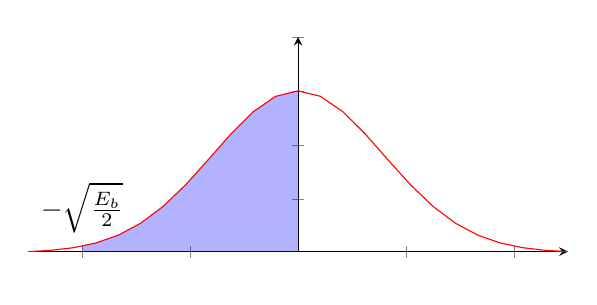
\begin{tikzpicture}
        \begin{axis}[
            unit vector ratio*=1 1 1,
            xticklabel=\empty,
            yticklabel=\empty,
            axis lines = middle,
            ymax = 4
            ]
            \addplot[color=red, name path = gauss] {3*exp(-((x)^2)/5)};

            \path[name path=axis] (axis cs:-4,0) -- (axis cs:0,0);
            \node [ label=$-\sqrt{\frac{E_b}{2}}$] at (axis cs: -4,0){};
            \addplot[color =blue, fill opacity =0.3]
                fill between [
                of = gauss and axis,
                soft clip = {domain=-4: 0}];
        \end{axis}
    \end{tikzpicture}

    (X: Da controllare su slide)
\end{minipage}
\begin{minipage}{0.5\textwidth}
\[ P_e = \int^0_{-\infty} \frac{1}{\sqrt{2\pi \sigma^2}} e^{-\frac{(n - \sqrt{E_b})^2}{2\sigma^2}}dn =\]
\[ = \int^{-\sqrt{E_b}}_{-\infty}\frac{1}{\sqrt{2\pi \sigma^2}} e^{-\frac{n^2}{2\sigma^2}}dn =\]
\[ \textit{Per Simmetria} \rightarrow = \int^{+\infty}_{\sqrt{E_b}}  \frac{1}{\sqrt{2\pi \sigma^2}} e^{-\frac{n^2}{2\sigma^2}}dn =\]
\[\framebox{\(\begin{split}
    z = \frac{n}{\sigma}\\
    \sigma dz = dn
    \end{split} \)} \rightarrow =
    \int^{+\infty}_{\frac{\sqrt{E_b}}{\sigma}}  \frac{\cancel{\sigma}}{\sqrt{2\pi \cancel{\sigma^2}}} e^{-\frac{z^2}{z}}dz =\]
\[ = \frac{1}{2} \erfc\left(\sqrt{\frac{E_b}{2\sigma}}\right)\]
\end{minipage}

Per simmetria, stessi calcoli per $-\sqrt{E_b}$, Quindi:
\begin{itemize}
    \item Trasmetto $-\sqrt{E_b}$ ricevo $+\sqrt{E_b}$:
        \[ P_e \big|_{-\sqrt{E_b}} = \frac{1}{2} \erfc\left(\sqrt{\frac{E_b}{2\sigma}}\right)\]
    \item Trasmetto $+\sqrt{E_b}$ ricevo $-\sqrt{E_b}$:
        \[ P_e \big|_{+\sqrt{E_b}} = \frac{1}{2} \erfc\left(\sqrt{\frac{E_b}{2\sigma}}\right)\]
\end{itemize}
Siccome sono due eventi indipendenti:
\[ P_{-E_b} = P_{+E_b} = \frac{1}{2} \]
\[ P_e = P_e \big|_{-E_b} \cdot P_{-E_b} + P_e \big|_{+E_b} \cdot P_{+E_b}= \frac{1}{2} \erfc\left(\sqrt{\frac{E_b}{2\sigma}}\right) \]


\subsection{Determinare Simbolo ricevuto da QPSK}
(x: Grafico simbolo)
Chiamato $r$ il simbolo ricevuto
\[ R = S+N \]
\[ \text{con} \quad S \in {s_1, s_2, s_3, s_4 } \qquad P{S = s_i} = \sqrt{1}{4}\]
\[ N \sim \mathcal{N}_{\mathbb{C}}(0, \sigma^2)\]

Ricevuto $R=r$, il problema diventa trovare il simbolo ($\bar{s}$) che minimizzi la probabilit\'a d'errore

\[ \bar{s} = s_i \quad \text{t.c.} \quad i = \argmax_{j \in 1\ldots 4} P\{ S=s_j \big| R=r\}  = \]
Per la formula di Bayes Mista:
\[= \argmax_{j \in 1\ldots 4} \frac{f_R(r | S=s_j) P\{ S=s_j\}}{f_R(r)} =\]
Dato che gli altri termini non dipendono da $j$:
\[= \argmax_{j \in 1\ldots 4} f_R(r|S=s_j) =\]
$R = S+N \rightarrow R$ \'e gaussiana a media $s_j$
\[ = \argmax_{j \in 1\ldots 4} \frac{1}{\sqrt{2\pi\sigma^2}} e^{-\frac{(r - s_j)^2}{2\sigma^2}} \]
Siccome $\exp$ \'e strettamente crescente:
\[= \argmax_{j \in 1\ldots 4} -(r - s_j)^2 = \framebox{$\argmin_{j \in 1 \ldots 4} | r - s_j |$} \leftarrow\text{Distanza Euclidea}\]

\section{Wired vs Wireless}
Utilizzando gli stessi approcci di una rete cablata, su una rete wireless, si manifestano due principali problemi:
\begin{itemize}
    \item Sul Wireless la Banda \'e molto pi\'u ridotta
    \item Il canale \'e pi\'u soggetto a fading che collision tra frame
\end{itemize}

Soluzioni:
\begin{itemize}
    \item TDMA: Reserves time slots
    \item FDMA: Reserves Frequencies
    \item CDMA: Reserves Expansion Codes
    \item Random Access Techniques
\end{itemize}

\subsection{FDMA}
Frequency Division Multiple Access: Utenti suddivisi in frequenza
\subsubsection{FDD}
Frequency division Duplex: Uplink e Downlink divisi in frequenze

(X: Grafico)

Pi\'u suscettibile ad interferenze in frequenza
\[ N_{\textit{max}} = \frac{B}{B_c K} \]

\subsubsection{TDD}
Uplink e Downlink divisi in intervalli di tempo

(X: Grafico)

\subsection{TDMA}
Time Division Multiple Access: Ad ogni utente \'e assegnato uno slot di tempo

(X: I due grafici)

\subsection{CDMA}
Code Division Multiple Access: Assegna ad ogni utente una sequenza di chip specifica e unica

\underline{Es}: Maximal length sequences $\rightarrow$ Periodiche con periodo $2^m -1$

Chiamato $x(n)$ un segnale (discreto) periodico

\begin{minipage}{0.5\textwidth}
\[ r_{xx}(l) = \sum^{2^m-1}_{n=0}  x(n)\dot x(n -l)\]
\[ r_{xx}(0) = \sum^{n-1}_{n=0} x^2(n) = 2^m \]
\end{minipage}
\begin{minipage}{0.5\textwidth}
    (X: Grafico coi punti)
\end{minipage}

$r_{xx}(1)= 0$ Siccome mediamente il numero di $+1$ \'e uguale al numero di $-1$

\subsection{DSSS Modulation}
Direct Sequence Spread Spectrum

Chiamata $m(t)$ la sequenza di bit da trasmettere

\[S(t) = \sqrt{\frac{2E}{T}} m(t)\cos(2\pi f_c t + \theta) = \sqrt{E}\,m(t)\sqrt{\frac{2}{T}}\cos(2\pi f_c t + \theta)\]

Schematizzato:

(X: Schema modulazione)

\[r(t) = m(t)p(t)\sqrt{\frac{2E}{T}}\cos(2\pi f_c t) + A_{int}(t) \]
\[p(t)r(t) = \cancel{p(t) p(t)}m(t) \sqrt{\frac{2E}{T}}\cos(2\pi f_c t) + p(t)A_{int}(t)
= \sqrt{\frac{2E}{T}}\cos(2\pi f_c t) + p(t)A_{int}(t) \]

Se N utenti vogliono trasmettere informazioni assegno ad ogniuno id essi un codice di spreading \underline{unico}

(Assumendo che tutti gli N codici di spreading siano quasi ortogonali tra di loro: $r_{xy} = 0$ nell'autocorrelazione con $x \ne y$

\( S_N(t) = \sum^N_{i=1} = m_i(t)p_i(t)s(t)\), Per ottenere $m_k(t)$, basta moltiplicare per il corrispettivo codice di spreading $p_k(t)$

\[ p_k(t) m_k(t) + \sum^N_{i \neq k} m_i(t)\cancelto{\approx 0}{p_i(t)p_k(t)}s(t) \]

\subsection{Vantaggi del CDMA}
\begin{itemize}
    \item Mis different users without any specificcoordination
    \item Nodes doesn't need to be syncronized
    \item Strong against noise
\end{itemize}
\subsubsection{Numero utenti supportati dal CDMA}
\begin{minipage}{0.5\textwidth}
    \[ \snr = \frac{P_S}{P_{th} + P_{int}} \]
\end{minipage}
\begin{minipage}{0.5\textwidth}
    \begin{itemize}
        \item $P_S$: Potenza di Segnale
        \item $P_{int}$: Potenza Interferenza
        \item $P_{th}$: Potenza termica = $FKT_0R_b$
            \begin{itemize}
                \item F Noise figure
                \item K Costante di Boltzmann $= 1.38 \cdot 10^{-23}$
                \item $T_0$ Temperatura Ambiente $= 290K$
                \item $R_b$ Bit Rate
            \end{itemize}
    \end{itemize}
\end{minipage}

\[ \snr \approx \frac{P_S}{P_{int}} = \frac{g P_r}{(N+1) P_r} \xrightarrow{N \gg 1} \frac{g}{N} = \frac{B}{R_b N} \]

Se viene richiesta una $\snr$ minima

\begin{minipage}{0.5\textwidth}
\[
    \begin{cases}
        \snr \ge \snr_{min}\\
        \snr = \frac{B}{R_b N}
    \end{cases} \Rightarrow N_{max} = \frac{B}{R_b \snr_{min}}
\]
\end{minipage}
\begin{minipage}{0.5\textwidth}
    \begin{itemize}
        \item $N$: Numero di interferenze
        \item $B$: larghezza della banda $=gR_b$
        \item $P_r$: Potenza ricevuta
        \item $g$: Spreading factor ($> 1$)
    \end{itemize}
\end{minipage}

$N_{max}$ \'e il massimo numero di utenti attivi contemporaneamente, \'e possibile migiorare le prestazioni del CDMA, modificando la disposiizone delle antenne trasmettitrici

\begin{minipage}{0.5\textwidth}
\[ N_{max} = \frac{B}{R_b \snr_{min}} K \qquad \text{con} \quad K = \frac{G_A G_\nu}{H_0}\]
\end{minipage}
\begin{minipage}{0.5\textwidth}
    \begin{itemize}
        \item $H_0$ Interferenza antenne vicine
        \item $G_A$ Sectorization Gain factor
        \item $G_\nu$ Voice activity factor $\approx 2.5$ (pause nella conversazione)
    \end{itemize}
\end{minipage}

\section{Rumore Termico}
Bianco, a media nulla

\begin{minipage}{0.3\textwidth}
    \begin{center}
    \begin{circuitikz}
        \draw (0, 0) to[R, o-o, l=$R$, v=$V$] (0, 2.5);
    \end{circuitikz}
    \end{center}
\end{minipage}
\begin{minipage}{0.2\textwidth}
    \[\bar{V} = 0\]
    \[ V^2 = \frac{2\theta^2 K^2 T^2}{3h}T \]
\end{minipage}
\begin{minipage}{0.5\textwidth}
    \begin{itemize}
        \item $R$: Resistenza
        \item $K$: Costante di Boltzman $1.37 \cdot 10^{-23}$ [$\frac{W_s}{K}$]
        \item $h$: Costante di plank $6.62\cdot10^{-34}$ [$Ws^2$]
        \item $T$: temperatura [$K$]
    \end{itemize}
\end{minipage}

$V$ ha una distribuzione Gaussiana:
\[ \bar{V} = 0 \]
\[ \bar{V^2} = \text{VAR}[V] \]

$S_V(f)$: (Densit\'a spettrale) \'e approssimabile ad una costante fino a valori di $f \approx 10^{12}Hz$

Da un punto di vista ingegneristico:
\[ S_V(f) \approx \frac{KT}{2} = \frac{N_0}{2} \]
Potenza di rumore:
\[ P = \cancel{2}B\frac{N_0}{\cancel{2}} = BN_0 = KT_0B \]

Banda di rumore equivalente su filtro con risposta $H(f)$:
\[ P_{N output}  = \int^{+\infty}_{-\infty} \frac{N_0}{2}|H^2(f)| df\]

$B_{eq} \coloneqq$ Banda di un filtro con risposta in frequenza rettangolare, ed in uscita la stessa potenza di rumore
\[ P_{N out} = B_{eq} \cdot \frac{N_0}{2} \]

Eguagliando le due espressioni otteniamo che:

\[ B_{eq} \cancel{\frac{N_0}{2}} = \int^{+\infty}_{-\infty} \cancel{\frac{N_0}{2}} | H(f) | df \]

Temperatura Equivalente di Rumore: Varie sorgenti di rumore si comportano similmente al rumore termico

\[ F(f) = \frac{S_{nf}(f)}{G S_{ni}(f)} \rightarrow F = \frac{P_{no}}{G P_{ni}}\]

\[
\begin{cases}
    G P_{Ni} F = P_{No}\\
    P_{No} = (P_{Ni} + kT_eB)G
\end{cases}
\]
\[ \cancel{G} P_{Ni} F = (P_{Ni} + KT_e B) \cancel{G} \]
\[ F = \frac{P_{Ni} + kT_e B}{P_{Ni}} = \frac{\cancel{k}T_0\cancel{B} + \cancel{K}T_e\cancel{B}}{\cancel{k}T_0\cancel{B}} = \frac{T_0 + T_e}{T_0} \leftrightarrow T_e = T_0 (F-1)\]

\section{Confronto fra T/F/C-DMA}
\begin{itemize}
    \item \textbf{TDMA} \'e pi\'u flessibile del \textbf{FDMA}, siccome il numero di utenti non \'e fissato a priori
    \item \textbf{TDMA} ha problemi di sincronizzazione tra gli utenti che devono trasmettere
    \item \textbf{CDMA}, Numero di utenti non \'e prefixxzto, basta associare ad ogniuno di essi una QoS (Quasi ortogonal Spread signal)
    \item \textbf{FDMA} lavora con bande molto strette $\rightarrow$ molto susciettibile a forti disturbi a breve frequenza
    \item \textbf{CDMA} pi\'u resistente alle forti interferenze su breve frequena, siccome vengono ``schiacciate'' dalla sequenza di spreading
\end{itemize}
\subsection{Handoff comparison}
\begin{itemize}
    \item \textbf{FDMA}: Brusco cambio di frequenza con la quale si trasmette
    \item \textbf{TDMA}: Mobile assisted Il client informa la BSC su come cambia il segnale
    \item \textbf{CDMA}: Entrambe le celle usano la stessa frequenza, se viene mantenuto lo stesso codice di spreading non ci sono problemi
    \end{itemize}

%% -- Section --
\newpage
\section{Random Access Protocols}

Tutti i protocolli ad accesso multiplo trasmettono su un unico canale.

Nal caso in cui due o piu nodi trasmettano contemporaneamente avviene una collisione.

Per comunicare, i nodi possono utilizzare solamente il canale

In una rete tra computer, non tutti i nodi trasmettono continuamente, quindi partizionare equamente le risorse del canale renderebbe la rete non del tutto utilizzata

\underline{Idealmente}: se il Broadcast channel ha una bit rate R
\begin{enumerate}
    \item Quando M nodi vogliono trasmettere, lo fanno con bit-rate \(\frac{R}{M}\)
    \item Decentralizzata: Non ci deve essere uno a coordinare le trasmissioni; i nodi non dovrebbero essere sincronizzati
\end{enumerate}

\subsection{Algoritmo ALOHA}

\subsubsection{Aloha Pure}
Pros:
\begin{itemize}
    \item No sincronization needed
\end{itemize}
Procedure:

\begin{enumerate}
    \item When new frame is received transmit it immediately
    \item on collision retry after a random interval
\end{enumerate}


\subsubsection{Aloha Slotted}
\begin{figure}[h]
    \centering
    
\includegraphics[width=1.8in]{placeholder.jpg}
    \caption{Slotted aloha}
\end{figure}
Assumptions:
\begin{enumerate}
    \item All frames have the same size
    \item Time is divided in equal slots
    \item Nodes transmit frames only at the beginning of a slot
    \item syncronization is needed
    \item Collision are always detected
\end{enumerate}


Procedure:

\begin{enumerate}
    \item New frame received transmit
    \item while no collisions are detected send next slot
    \item If collision: start transmission in the next slot with probability P until success
\end{enumerate}
\hfill

\newpage
\section{Protocollo Ethernet CSMA/CD}

\textbf{CSMA/CD}: Carrier Sense Multiple Access, Collision Detection

Si basa sul fatto che le collisioni tra pacchetti vengono riconosciute ed individuate in poco tempo. Quando ne avviene una, la trasmissione del pacchetto viene interrotta.

Dato che il segnale si propaga su un cavo, per determinare le collisioni basta confrontare l'energia del cavo ricevuta, con la potenza di un segnale trasmesso, per poter identificare facilmente un interferenza.

Questo metodo \`e molto efficente soprattutto se le dimensioni del pacchetto sono molto pi\'u lunghe rispetto ai tempi di propagazione.

Purtroppo, non \'e possibile utilizzare lo stesso sistema di error-detection nelle reti wireless, dato che la potenza del segnale ricevuto dipende molto dalla distanza tra gli utenti e la sorgente del segnale, quindi non sempre una bassa potenza di segnale implica l'assenza di collisioni.

\subsection{Struttura di un frame Ethernet}

Struttura frame livello 2:
\begin{itemize}
    \item \textbf{Preamble}: [8 byte] 7 con pattern 10101010, ed 1 con 10101011; Utilizzati per sincronizzare il ricevitore e trasmettitore
    \item \textbf{Destination \& Source Address}: [6 byte] Target machine / Broadcast \& Source machine MAC Address
    \item \textbf{Type}: Protocollo di livello 3 (ex: IP)
    \item \textbf{CRC}: Cycling Redundance Check; Controlla solo se si sono verificati errori, non si occupa della correzione.

        In caso di errore tutto il frame viene scartato
\end{itemize}

\subsection{Ethernet (Standard IEEE 802.3)}

CSMA/CD 1 Persistent:

Aspetta fino a quando il canale \'e libero, dopo trasmette immediatamente (\textit{1 Persistent}).
Quando si verifica una collisione, viene trasmesso un segnale ad alta energia chiamato \textit{Segnale di JAM} (\textit{JAM Signal}).

\subsection{Collision Detection}

Per assicurarsi che le collisioni vengano individuate, \'e richiesto che $2T$ (\textit{Round Trip Time}) sia al pi\'u $51.2\mu s$.
Da cui, supponendo che si trasmetta a $10Mbps$, la lunghezza di un pacchetto minima deve essere $64b$.

In questo modo ci si assicura che tutti gli host notino la collisione.

\subsection{Binary Exponential Backoff}
In caso di $N$ collisioni consecutive viene generato un numero casuale $K$ compreso tra $0$ e $2^N$, chiamata $T_s$ l'unit\'a di tempo, prima di trasmettere di nuovo un pacchetto vengono aspettati $K T_s$ secondi.

$T_s = 51.2\mu s$ per il protocollo Ethernet $802.3$

\subsection{Efficenza}
In condizioni di saturazione:

$t_{prop}$: Tempo massimo di propagazione tra due Nodi nella rete ($T_s$)

$t_{trans}$: Tempo di trasmissione massima di un frame ($1.2 ms$), calcolato come $t_{trans}\frac{D_p}{R}$ ($D_p$ dimensione pacchetto, $R$ bit rate).

\[Eff \approx \frac{1}{1 + 5\frac{t_{prop}}{t_{trans}}} \approx 82.6\%\]

\subsection{Recezione dei Frame}
Ethernet controller card si occupa di filtrare i frame destinati all'host rispetto a tutti i pacchetti nella rete

Transceiver (Utilizzato nelle reti con topologia a bus) si occupa di:
\begin{itemize}
    \item Carrier detection
    \item Collision detection
    \item Jamming
\end{itemize}

Nelle reti con topologia ad hub (stella), i singoli host si occupano di Carrier detection, l'hub centrale di:
\begin{itemize}
    \item Collision detection
    \item Jamming
\end{itemize}

\section{WiFi CSMA/CA 802.11}
Collision Sense Multiple Access/Collision Avoidance


\begin{enumerate}
    \item Se il canale \'e occupato e devo trasmettere un frame, Cronometro quanto il canale ci impiega a tornare libero, chiamo questo tempo $T$.
    \item Appena il canale si libera, prima di trasmettere il frame aspetto lo stesso tempo $T$
    \item Se il canale torna occupato prima che finisca il mio `countdown', interrompo il `countdown' e lo riprendo appena il canale torna livero.
    \item Altrimenti trasmetto il frame Immediatamente
\end{enumerate}


\subsection{Hidden and Exposed Terminal Problems}
Avviene nel caso in cui due o pi\'u nodi riescono a trasmettere alla base station, ma il loro segnale non \'e abbastanza forte da individuarsi a vicenda.
Per questo motivo, se uno dei due fa \textit{Carrier Sense}, non individua l'altro, e, trasmettendo contemporaneamente generano interferenza alla base station.

\textbf{Soluzioni}:
\begin{itemize}
    \item Busy Tone Multiple Access (BTMA): la banda viene divisa in due, una sottobanda viene utilizzata per la trasmissione dati, l'altra per capire quando trasmettere
    \item Request-To-Send/Clear-To-Send (RTS/CTS): coppia di messaggi di handshake tra device e base station, utilizzati per `detect' di trasmissioni vicine.
\end{itemize}


\subsection{Wi-Fi Trivia}
\textbf{Wi-Fi}: Wireless Fidelty

\textbf{Wi-Fi Alliance}: Organizzazione non-profit che ha creato il brand ``Wi-Fi'', di cui sono parte molte aziende. Il logo garantisce la compatibilit\'a dei dispositivi con i protocolli ethernet e Wi-Fi.


\subsection{Standard 802.11b}
Utilizza la banda a $2.4 GHz$, soggetta ad interferenze da altri device (come microonde, telefoni cordless..), suddivisa in 11 canali, di cui solo 3 non sovrapposti.

Supporta un data rate massimo idealmente da 1 a 11$Mbps$, ma realisticamente da $4-5Mpbs$ al massimo.

Utilizza il protocollo $DSSS$

\subsection{Standard 802.11g}
Utilizza sempre la banda a $2.4GHz$, ma ha un raggio di trasmissione pi\'u corto rispetto a \textit{802.11b}. \'E compatibile ancora con lo standard \textit{802.11b}.

\`E piu flessibile siccome cnali multipli possono essere combinati per aumentare il thrughput, ma rimane limitato ad un unico access point.

Idealmente ha un massimo di $54 Mbps$, ma realisticamente $20-25 Mbps$ e $14 Mbps$ se associato con \textit{802.11b}

Utilizza FDD
\subsection{Standard 802.11a}

Come \textit{802.11g} pi\'u canali possono essere utilizzati per aumentare il thrughput, ma non rimane limitato ad un unico access point.

Il raggio di trasmissione \'e piu corto degli altri due protocolli precedenti.

Utilizza FDD con banda a $5GHz$, ed ha 12 canali, di cui 8 non sovrapposti. Raggiungendo una velocit\'a ideale dai 6 ai $54Mbps$ (Realisticamente $\approx 25 Mbps$)
\newpage
\section{Personal Area Network (PAN)}
Rete di device disposti a distanza ridotta ($\approx 1-10m$), pu\'o essere
\begin{itemize}
    \item Cablata: Connessa attraverso USB o BUS
    \item Wireless: Connessa utilizzando protocolli come Bluetooth, ZigBee, IrDA, etc.
\end{itemize}

Ha come vantaggio principale quello di richiedere poca energia.

Utilizza sempre la frequenza portante di $2.4GHz$

\section{Bluetoooth 802.15.1}
Ha come vantaggi principali:
\begin{itemize}
     \item ridotto costo
     \item Connessioni ad hoc
     \item Ideale per trasissione di dati vocali in tempo reale
     \item Rimuove la necessit'\'a di numerose porte, utilizzate per connessioni cablate
\end{itemize}

\subsubsection{Architettura del Protocollo}
Interfaccia \textbf{Audio} comunica direttamente con la banda base.

Banda base a 79 portanti, utilizza CDMA con hopping sequences, per minimizzare il danneggiamento del segnale provocato dal canale di comunicazione (Interferenza da cammino multiplo).

Nel caso non venga utilizzata l'inerfaccia audio, il Link Manager Protocol si occupa dell'autenticazione e crittografia del segnale trasmesso

SDP, Service Discovery Protocol, si occupa di individuare altri dispositivi che utilizzando bluetooth.

Ogni nodo ha un \textit{Bluetooth Device Address} (\textit{BD\_ADDR}). Il nodo Master determina tutte le frequenze di hopping dei nodi Slave.

Network topology organizzate in:
\begin{itemize}
    \item Piconet: Insime di nodi bluetooth sincronizzati con un unico master
    \item Scatternet: Insieme di piconet
\end{itemize}

All'interno di una rete, Master e Slaves possono invertirsi i ruoli

\subsection{Formato pacchetto bluetooth}
\begin{itemize}
    \item \textbf{Access Code}: [$72 bit$]
    \item \textbf{Packet Header}: [$54 bit$] Contiene MAC Address, ed altri bit di controllo
    \item \textbf{Payload}: [$0-2745 bit$] Dati effettivi trasmessi
\end{itemize}

\subsection{Possibili stati di un dispositivo bluetooth}
\begin{itemize}
    \item ACTIVE:  Unicamente identificato da un AM\_ADDR, e sta trasmettendo
    \item SNIFF: partecipa alla piconet nello SNIFF interval
    \item HOLD: Tiene solamente attiva la connessione
    \item PARK: (low-power): Rilascia il suo AM\_ADDRM, rinmanendo per\'o sincronizzato col master
\end{itemize}

BlueTooth device addressing:
\begin{itemize}
    \item BD\_ADDR [$48 bit$]
    \item AM\_ADDR [$3 bit$]: ACTIVE, HOLD or SNIFF
    \item PM\_ADDR [$8 bit$]: PARK MODE address, scambiato con AM\_ADDR quando si entra in PARK MODE
    \item AR\_ADDR [$8 bit$]: usato quando si passa dallo stato PARK a ACTIVE
\end{itemize}

\section{Protocollo LoRa}
Tecnologia (LPWAN: Low Power Wide Area Network), Bassto su modulazione CSS nel 2014

Utilizzato a livello industriale per connettere dispositivi (IoT),

Da tenere conto per protocolli utilizzati nell'IoT
\begin{itemize}
    \item batteria
    \item larga copertura
    \item sicurezza
    \item costo
\end{itemize}

\textit{LPWAN}: come reti cellulari ma ottimizzate per \textit{IoT/M2M}, (topologia a stella)

Caratteristiche:
\begin{itemize}
    \item Wide range
    \item Low power
    \item Low cost
    \item Low data-rate
    \item Unlicensed bands
\end{itemize}

LoRa \'e il livello fisico su cui LoRaWAN lavora; LoRa \'e il livello fisico

Comunicazinoe device-gateway in lora, gateway-network via ip

\subsection{livello fisico}
Modulazione basata su Chirp Spread Spectrum (CSS): Frequenza Aumenta Progressivamente

Spreading Factor: Quanto un simbolo viene ``allargato'' nel tempo, ogni volta che viene incrementato di 1, raddoppia il tempo di trasmissione ed il consumo di energia

\subsubsection{Composizione frame LoRa}
\begin{enumerate}
    \item Preambolo, serve a stimare la frequenza utilizzata e la qualit\'a del canale
    \item  Inizio della data Unit di livello fisico: Il dispositivo comunica la fine del preambolo per iniziare a trasmettere i dati
    \item  dati
\end{enumerate}

Air Time: Quanto deve stare acceso il chip per trasmettere dei dati

$T_{off}$ Duty Cycle: Tempo che `devo stare zitto' dopo aver trasmesso (Duty Cy
\[ T_{air} = T_S (n_{preamble} + n_{payload} + 4.25 )\]
\[ T_{off} = T_{air} \left( \frac{1}{d} -1 \right) \]

\subsubsection{Capture Effect}
Fenomeno associato con FM reception, dove solo il segnale pi\'u forte ( o pi\'u vicino) sar\'a demodulato

\subsection{Livello MAC (LoRaWAN)}
% Da slide 54
TTN: Server di rete

Esistono 3 tipi di classi
\begin{itemize}
    \item \textbf{A}: Sensori alimentati a batteria (A sta per supportati da \underline{all} devices) pi\'u efficenti dal punto di vista energetico, uplink regolato da Aloha
    \item \textbf{B}: (Attuatori alimentati a batteria) \underline{Beacon}, sincronizzazione tra nodi e gw tramite beaco
    \item \textbf{C}: Attuatori alimentati a rete elettrica in \underline{Continuous} listening
\end{itemize}

Per i dispositivi di classe A c'\'e una finestra di downlink dopo ogni trasmissione; Dopo $t_1$ secondi, apre una receiving slot a stessa frequenza e spreading factor della trasmissione

Se riceve un pacchetto di downlink finisce la trasmissione col gateway

Se non lo riceve, dopo $t_1 + 1$ secondi apre una nuova frequenza di trasmissione con SF e altro prestabiliti

Siccome utilizza Slotted Aloha ci deve essere una perfetta sincronizzazione tra end-device e gateway

Tra i messaggi pi\'u importanti trasmiessi ci sono i MAC Commands, utilizzati per impostare potenza, spreading factor $\ldots$


Adaptive Data Rate: Cambia Spreading factor per ottimizzare l'energia consumata, algoritmo attuale si basa su una stima dell'SNR dagli ultimi pacchetti ricevuti

\subsection{Architettura di rete e Sicurezza}
\begin{center}
(X: Immagine slide 63)
\end{center}

Quando un nodo trasmette, tutti i gateway nel range trasmissivo ricevono un pacchetto; \'e il server che sceglie quale pacchetto prendere in considerazione, in base alla potenza del segnale ricevuto

$\ldots$

Network server:
\begin{itemize}
    \item Gestisce le join
    \item Controlla che non ci siano pacchetti duplicati
    \item Decide a quale gateway inviare messaggio di downlink
\end{itemize}

Application Server: Riceve i pacchetti, schedula le risposte e decripta il payload

Per identificare i nodi univocamente:
\begin{itemize}
    \item DeviceEUI: Indirizzo a 64 bit come mac address
    \item DevAddr: indirizzo 32 bit generato da Network (Parallelo dell'IP)
    \item AppEUI: identificato univocamente
    \item Fport: Identifica univicamente (App/server) parallelo di TCP/IP
\end{itemize}

% Schema slide 74: Come avviene la cifratura (AES a 128b)
% 75: integrity check (server conosce tutte le chiavi di sessione)

\subsection{Concludendo}

\begin{itemize}
    \item Lunghe distanze
    \item Lunga durata della batteria
    \item cheap devices
    \item infrastruttura semplice
\end{itemize}

Scalabilit\'a ridotta

$\ldots$
\section{ZigBee 802.15.4}
Ideato specialmente per low-rate low-power PANs.

Basato sul `\textit{Garantire time slot ai device nella rete}'


\textbf{Beacon-Enabled Mode}: La sincronizzazione tra nodi si effettua tramite pacchetti \textit{beacon}, il tempo disponibile viene suddiviso in superframe. Maggiore complessit\'a nei songoli nodi.

\textbf{Beaconless Mode}: Nessuna sincronizzazione tra nodi, minore complessit\'a nei singoli nodi ma meno efficente rispetto a beacon-mode.

\subsection{Topologia rete}
I nodi sono raggruppati in PAN, identificate da un \textit{PAN ID}.

Almeno uno dei nodi presenti in ogni PAN, ha il ruolo di coordinatore: Organizza l'inizializzazione dell'intera pan (es. Configurazione del PAN ID), l'associazione dei nodi e delle trasmissioni dei beacon.

Nodi aggiuntivi della rete sono chiamati \textit{end-devices}.

Tutti i nodi sono divisi logicamente in FDD (Full Function Devices) e RFD (Reduced Function Devices). FFD implementano tutte le funzionalit\'a ZigBee e possono comunicare con tutti gli altri nodi nel range trasmissivo

Tutte le topoligie permesse contengono almeno un Coordinatore di rete, e gli RFD, possono essere solamente foglie del grafo, mentre gli FFD possono essere rami o foglie.

Viene utilizzato una low-transmission rate: $20-40 kbps$

%TODO: Modulation slide 209 210
% specifications & allowed topology

\subsection{Struttura pacchetto}
\begin{itemize}
    \item Beacons: usato dal PAN coordinattor
    \item Data: Usato dai livelli pi\'u alti per trasferire dati
    \item Achknowledgement: Usato per confermare la corretta recezoine del pacchetto
    \item MAC command: manage all control information
\end{itemize}

Utilizza il protocollo CSMA/CA unslotted.
Tempo d'attesa generato casualmente sull'intervallo $[0, 2^{BE} - 1]$

\subsection{Network Topologies}
\begin{itemize}
    \item Star: no router solo un padre
    \item Tree: Coordinatore della PAN \'e la radice, i router possono diramarsi in router o end device. (energy efficient)
    \item Mesh: Tutti i nodi possono comunicare, (non applicabile beacon mode)
\end{itemize}

\section{Cellular Network Dimensioning}


Aumentare $K$ ha un impatto sul numero di risorse frequenziali assegnate ad ogni cella.

Le risorse frequenziali sono strettamente legate al numero di utenti gestibili.
$+K$ a parit\'a di area di cella, meno densit\'a geografica degli utenti

\subsection{Handover/Handoff}

Handover non assistito: gestito da BTS adiacenti

Handover assistito da Mobile station: Mobile Station genera informazioni di controllo per una gestione migliorata dell'handover.

\subsection{Dimensionamento rete cellulare}

$A_{cella} \coloneqq$ Area di una singola cella

Tutte le celle hanno la stessa dimensione. (Non vero per $5G$)

Un Area coperta da una cella richiede maggiore potenza trasmissiva.

Supponendo che $M_{cella}$ sia il numero di risorse frequenziali assegnate ad ogni cella, la densit\'a geografica degli utenti \'e calcolata come:
\[ u = \frac{M_{cella}}{A_{cella}} \]

Chiamato $M$ il numero complessivo di risorse a disposizione, e $K$ le dimensioni del Kluster:
\[ M_{cella} = \frac{M}{K} \]

Chiamato $R$ il raggio della cella associata dell'esagono.
\[ A_{cella} = \frac{6}{2}R^2\frac{\sqrt{3}}{2} \quad \rightarrow \quad
    u=\frac{M}{K}\frac{2}{3\sqrt{3}R}
\]

Maggiore \'e il numero di risorse a disposizione, maggiore \'e il numero di utenti gestibili per $Km^2$

\textbf{Distanza di riuso} ($\mathcal{D}$): Distanza tra centri di celle analoghe

\underline{Sperimentalmente} i valori che $K$ pu\'o assumere non snono arbitrari, ma devono rispettare la relazione
\begin{minipage}{0.5\textwidth}
\[ K = i^2 + j^2 + ij \qquad\quad
    \begin{cases}
    i,j \in \mathbb{N} \\
    i+j \neq 0
    \end{cases}
\]
\end{minipage}
\begin{minipage}{0.3\textwidth}

\begin{center}
\begin{tabular}{c c|c}
    i & j & k\\
    \hline{}
    0 & 1 & 1\\
    0 & 2 & 4\\
    0 & 3 & 9\\
    1 & 1 & 3\\
    1 & 2 & 7\\
    1 & 3 & 13\\
    1 & 4 & 21\\
    2 & 2 & 12\\
    2 & 3 & 19\\
    2 & 4 & 28\\
    3 & 3 & 27\\
\end{tabular}
\end{center}
\end{minipage}

Partendo dal centro di una cella, si arriva ad una cella analoga seguendi i passaggi:
\begin{enumerate}
    \item Muoversi $i$ celle seguendo una direzione perpendicolare ad un lato dell'esagono di partenza
    \item Ruotarsi di $\frac{2}{3}\pi$ in senso (anti)orario
    \item Muoversi di $j$ celle seguendo il verso della rotazione
\end{enumerate}

La formula della distanza di riuso tra 3 celle, si calcola (utilizzando il Teorema di Carnot):

\[
\begin{aligned}
    \mathcal{D} &= \sqrt{(i\sqrt{3}R)^2 + (j\sqrt{3}R)^2 - 2(i\sqrt{3}R)(j\sqrt{3}R)\cos({\textstyle \frac{2}{3}}\pi) } = \\
                &= R\sqrt{3i^2 + 3j^2 + 3ij} = \sqrt{3}R\sqrt{i^2 + j^2 + ij} = \framebox{$\sqrt{3K}R$}
\end{aligned}
\]

\subsection{Interferenza tra celle adiacenti (Downlink)}
\begin{wrapfigure}{R}{0.4\textwidth}
    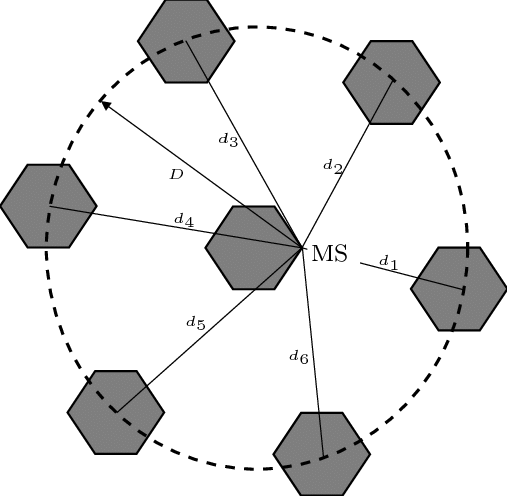
\includegraphics[width=0.4\textwidth]{img/sdt/bts_interferenti}
    \centering
    \caption{Disposizione BTS Interferenti\label{bti}}
\end{wrapfigure}

Definiamo la qualit\'a del segnale come:
\[ Q \coloneqq \frac{D}{R} = \sqrt{3K} \]
Siccome \'e schematizzata ad esagono (Figura~\ref{bti}), ci sono al massimo 6 segnali interferenti

$ C = \frac{\chi}{R^n}$: Potenza segnale ricevuto (da formula di Friis)

\[ I_i = \frac{\chi}{d_i^n} \approx \frac{\chi}{\mathcal{D}^n}\]

La distanza dipende dalla cella, $d_{i_{max}} = d_i + r$, mediamente $d_i \approx \mathcal{D}$. Possiamo sovrastimare la potenza di Interferenza complessiva $I$ come:

\[I \le \sum\limits^6_{i=1} I_i = 6\frac{\chi}{\mathcal{D}^n}\]

\`E uguale se tutte le celle analoghe di $1^a$ fascia stanno utilizzando la stessa risorsa. Minore se almeno una delle celle analoghe non utilizza la stessa risorsa

\[
    \snr=\frac{C}{I} \ge \frac{\frac{\chi}{R^n}}{6\frac{\chi}{\mathcal{D}^n}} =
    \frac{1}{6}{\left(\frac{\mathcal{D}}{R}\right)}^n =
    \frac{1}{6}Q^n = \frac{{(\sqrt{3K})}^n}{6}
\]

Per aumentare $\snr$ in downlink, considero invece di un antenna omnidirezionale, 3 antenne direttive, ogniuna con diagramma di irradiazione di $120^\circ$. Ad ogniuna delle 3 antenne \'e assegnato $\frac{1}{3}$ delle risorse della cella.

In questo modo:
\[ {\left(\frac{C}{I}\right)}_{dl}  \ge \frac{a^n}{2} = 3\cdot\frac{a^n}{6}\]

In generale su celle tri-settoriali il rapporto aumenta di un fattore compreso tra 2 e 3. Ma comporta un handover sui settori della stessa cella. Al fine di evitare questi costi, si possono considerare siti 3-settoriali, ma richiedono che $K$ sia multiplo di 3.

%TODO Disegno celle trisettoriali
(X: Disegno Trisettoriale)

\subsection{Calcolo C/I Uplink}
Utilizziamo come \textbf{assunzione peggiorativa} che la Mobile Station \'e a distanza $R$ dalla BTS.

(X: Disegno posizioni)

Inoltre (\textbf{assunzione peggiorativa}) la mobile station che pu\'o interferire \'e pi\'u vicina possibile ala BTS, \'e eattamente a ditanza $\mathcal{D} - R$, questo implica che la retta che unisce i due centri delle BTS passa per uno spigolo.

\[I_i = \frac{\chi}{d_i^n} \]

considerando l'$I_i$ legata ad una singola Mobile station nella cella
\[ I = \sum\limits_{i=1}^6 \approx 6\frac{\chi}{{(\mathcal{D} - R)}^n} \]

\[ C = \frac{\chi}{R^n} \quad,\quad {\left(\frac{C}{I}\right)}_{up}
    = \frac{1}{6}\frac{{(\mathcal{D} - R)}^n}{R^n}
    = \frac{1}{6}\left(\frac{\mathcal{D}}{R} -1 \right)^n = \frac{1}{6}(Q - 1)^n
\]

\subsection{Considerazioni Finali}
\begin{center}
\begin{tabular}{c|c|c}
    & $R\uparrow$ e $K$ cost & $R$ cost e $K\uparrow$\\
    \hline
    Potenza trasmissiva  & {\color{red}$\nearrow$}  & -\\
    Numero di Handoff    & {\color{green}$\searrow$}& -\\
    Densit\'a geografica & {\color{red}$\searrow$}  & {\color{red}$\searrow$}\\
    Rapporto C/I         &                         -& {\color{green}$\nearrow$}
\end{tabular}
\end{center}

\section{GSM (2G)}
Global System for Moblile Communication. \`E organizzato in una struttura fortemente gerarchica.

Introduce per la prima volta sul mercato una trasmissione dati dii tipo digitale. Portando enormi vantaggi rispetto ai precedenti sistemi cellulari.
\begin{itemize}
    \item Pi\'u velocit\'a di trasmissione  grazie alle tecniche di compressione dei dati e codifica di sorgente.
    \item Introduzione delle funzioni di sicurezza e cifratura
    \item Introduce un grande numero di servizi grazie all'aumento della velocit\'a di trasmissione (es. SMS)
\end{itemize}

% GSM:\@\textit{Goup Special Mobil}\'e organizzato in stuttura fortemente gerarchica

\begin{wrapfigure}{R}{0.5\textwidth}
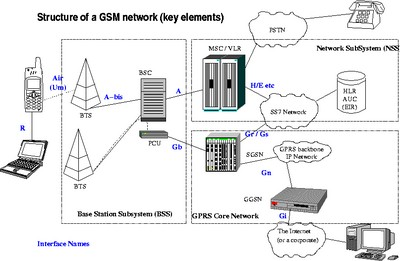
\includegraphics[width=0.5\textwidth]{img/sdt/architettura_uts}
\caption{Architettura GSM}
\centering
\end{wrapfigure}

\bigbreak
MSS:\@\textit{Mobile Station Subsystem}, Connessione alla rete via interfaccia radio

MMI:\@\textit{Man-Machine Interface}

HMI:\@\textit{Human-Machine Interface}

Access Network:
\begin{itemize}
    \item BTS: Base Transceiver Station
    \item BSC: Base Station Controller (Gestisce Handover)
\end{itemize}

Core Network:
\begin{itemize}
    \item MSC: Mobile Switching Center, commutazione circuito
    \item SGSN: Interfaccia commutaizione pacchetto
\end{itemize}


IMEI:\@\textit{International Mobile Equip Identity}

HLR:\@\textit{Home Location Register}, Database s cui un gestore GSM memorizza permanentemente i dati relativi agli utenti sottoscritti (IMSI, MSISDN)

VLR:\@\textit{Visitor Location Register}, Mantiene aggiornate le informazioni sulla mobile Station (IMSI, MSISDN, HLR, TMSI, Stato Mobile Station, Location Area Identity)

SIM:\@\textit{Subscriber Identity Module}, ha come scopo principale quello di fornire l'autenticazione ed autorizzazione per accedere alla rete. Non contiene all'interno il numero di telefono, perch\'e associato all' \textit{IMSI}. Contiene:

\begin{itemize}
    \item IMSI: \textit{International Mobile Subscriber Identity}, Numero univoco associato ad ogni utente, mandato da un dispositivo della rete (molto raramente) a HLR e VLR. Composto da:
        \begin{itemize}
            \item Utente
            \item Operatore
            \item Nazione
        \end{itemize}
        Per garantire riservatezza agli utenti viene inviato al suo posto un TMSI (\textit{Temporary MSI}) casualmente generato.
    \item Chiave segreta utilizzata sia per autenticare il chiamante sia per cifrare i dati.
    \item Memoria interna (Conentiene al massimo 256 Numeri di telefono)
\end{itemize}


\textit{Mobile Station International Subscriber Directory Number} (MSISDN): Identifica univocamente l'untente nel piano di numerazione della rete telefonica del gestore.

BSS:\@\textit{Base Station Subsystem}

\begin{itemize}
    \item BTS:\@\textit{Base Transceiver Station}: Hardware per recezione, antenne modem ed amplificatori
    \item BSC:\@\textit{Base Station Controller}: Gestisce canali radio delle BTS che controlla e mobile station collegate.

        Utilizza frequency hopping per prevenire trasmissione continua su canali `cattivi'

        Gestisce Handoff tra:
        \begin{itemize}
            \item Celle Adiacenti
            \item Stessa Cella
        \end{itemize}
\end{itemize}

TRAU:\@\textit{Transcoder Rate Adaptation Unit}, Adattatore codifica vocale usata con codice vocale in rete

Codifica sorgentte vocale telefono (RPE-LTP), compongono la voce ed elimina la ridondanza, campionando il segnale.

PCM:\@\textit{Pluse Code Modulation}

Voce campionata su smartphone, TRAU rigenera ridondanza
\subsection{Architettura rete GSM}
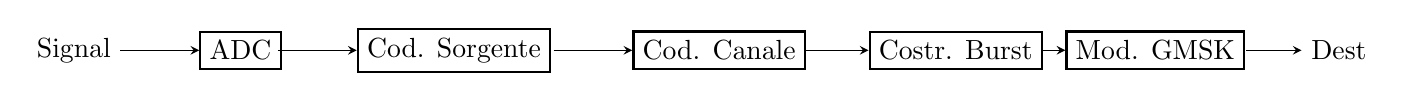
\begin{tikzpicture}
    [blocco/.style={rectangle ,thick ,draw }]
    \node[left] at (0,0) {Signal};

    \draw[-stealth] (0,0)--(1,0) node[blocco, right]{ADC};
    \draw[-stealth] (2, 0)--(3,0) node[blocco, right]{Cod. Sorgente};
    \draw[-stealth] (5.5, 0)--(6.5,0) node[blocco, right]{Cod. Canale};
    \draw[-stealth] (8.7, 0)--(9.5,0) node[blocco, right]{Costr. Burst};
    \draw[-stealth] (11.7, 0)--(12,0) node[blocco, right]{Mod. GMSK};
    \draw[-stealth] (14.3, 0)--(15,0);

    \node[right] at (15,0) {Dest};

\end{tikzpicture}

\begin{itemize}
    \item ADC:\@\textit{Analog Digital Converter}
    \item Codifica di sorgente: RPE-LTP (Regular Pulse Excitation Long Term Reduction)
    \item Codifica di Canale
    \item Codifica di Sorgente, Rate di codifica $\frac{1}{2}$: Ricevuto in ingresso 1 bit, inserisce ridondanza e manda 2 bit in uscita
    \item Costruttore di burst
    \item Destinazione
\end{itemize}

Bande in uplink: $\frac{890}{915} MHz \rightarrow$ Banda di coerenza $25MHz = B$

GSM lavora con sottobande di $200 KHz$ ($B_C$) $\rightarrow$ Numero di sottobande possibili: $\frac{B}{B_C} = \frac{25\cdot10^3 kHz}{200KHz} = 125$. Per essere sicuri di non `sforare' dalla banda a disposizione, ne vengono utilizzate solamente 124.

Ogni sottobanda viene indicata con un ARFCN (\textit{Absolute Radio Frequency Channel Number})

Ogni sottobanda pu\'o essere assegnata fino ad un massimo di 8 utenti. Viene utilizzato un TDMA a 8 slot per ogni sottobanda. Da cui il numero di utenti gestibili: $124*8 = 992$

Ogni time slot viene indicato con TSn

La coppia ARFCN-TSn indica univocamente una risorsa.

Se il \textit{`Passo di Duplice'} \'e costante, basta conoscere la sottobanda in uplink per identificare univocamente anche quella in downlink.

Il vantaggio di utilizzare l'ibrido FDMA/TDMA \'e la possibilit\'a di utilizzare il frequency hopping nel TDMA: Ad ogni utente non viene assegnata solamente una risorsa, ma una serie di risorse $\Rightarrow$ Riduzione danneggiamento comunicazione da sottobane danneggiate.

Per la modulazione del segnale viene utilizzata un GMSK (\textit{Gaussian Minimum Shift Keying}), Un formato di modulazione molto efficente.
\begin{enumerate}
    \item Efficenza spettrale superiore a $1 \textit{symbolo}{Hz}$
    \item Robusta contro l'evanescenza
    \item Ha un ampiezza costante, viene gestito in modo efficente amplificatori
    \item Semplice come implementazione
\end{enumerate}

\subsection{Struttura di uno slot GSM}
\begin{center}
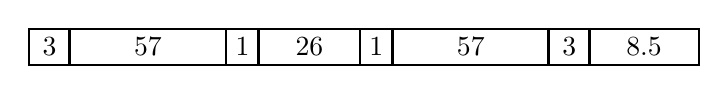
\begin{tikzpicture}
    [block/.style={rectangle, thick, draw}]
    \node[block] at (0,0) {$\,3\,$};
    \node[block] at (1.25,0) {$\qquad57\qquad$};
    \node[block] at (2.45,0){1};
    \node[block] at (3.3,0){$\quad26\quad$};
    \node[block] at (4.15,0){1};
    \node[block] at (5.35,0) {$\qquad57\qquad$};
    \node[block] at (6.6,0) {$\,3\,$};
    \node[block] at (7.55, 0){$\quad8.5\quad$};
\end{tikzpicture}
\end{center}

\textbf{Multiframe}: Composto da 26 frame, dura 120ms

Ogni \textbf{Frame} \'e composto da 8 slot

Ogni \textbf{Slot} dura $577\mu s$, ed \'e composto da 156.25 bit. Gli 8.25 bit terminali non vengono utilizzate nel frame, per evitare problemi con la sincronizzazione, in questo mod lo slot \'e simmetrico.


\begin{itemize}
    \item Bit di coda [3 bit]: principalmente utilizzati per consentire l'accensione e spegnimento dell'amplificatore di potenza.
    \item Campi dati [57 bit]: payload
    \item Stealing flag [1 bit]: quando vanno ad 1, i campi dati vangono utilizzati per il controllo.

        Utilizzati nelle operazioni critiche (handover, cambiaento arfcn-tsn)
    \item Midambolo
\end{itemize}

Il \textbf{midambolo} \'e noto al tramettotore ad al ricevitore.

\begin{center}
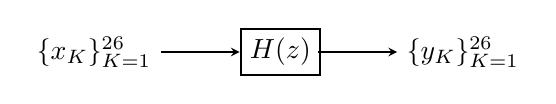
\begin{tikzpicture}
    [block/.style={rectangle, thick, draw}]
    \node[left] at (0, 0) {$\{x_K\}_{K=1}^{26}$};
    \draw[-stealth] (0,0)--(1,0) node[block, right]{$H(z)$};
    \draw[-stealth] (2,0)--(3,0) node[right]{$\{y_K\}_{K=1}^{26}$};
\end{tikzpicture}
\end{center}

Per trovare $h_k$ si usa la sequenza nota $y_k = x_k \oplus h_k$.

$h_k$: Channel Impulse Response

Dato che la risposta in frequenza del canale varia continuamente nel tempo, il modo migliore per stimarla \'e valutarla a met\'a del pacchetto.

$T_s \coloneqq$ Tempo di simbolo $ = \frac{\text{Durata slot}}{\text{Dimensione Pacchetto}} = \frac{577 \mu s}{156.25} \approx 3.69\mu s$

Banda di coerenza: $\frac{1}{5\sigma}$

Banda del segnale $=\frac{1}{3} \gg$ Banda di Coerenza $\approx \frac{1}{80}$

Su $200KHz$ la risposta in frequenza potrebbe essere quella (figura).

\textbf{Tempo di coerenza}: Legato all'effetto doppler; $f_D$ (Frequenza doppler) $\approx 100Hz$ nel GSM

\[ T_{coer} \approx \frac{9}{16\pi f_D} \approx 1ms \]

\[T_{burst} = T_{slot} = 577 \mu s = 0.57 ms \approx T_{coer}\]

\textbf{Risposa Trasmissiva} ($Rb$) $\approx \frac{114\cdot24}{120\cdot10^{-3}} = 22.8\frac{Kb}{s}$

\subsection{Gerarchia di Segnalazione GSM}
\begin{itemize}
    \item Burst-Slot: 577$\mu s$
    \item Frame (8 Slot): 4.65ms
    \item Multiframe (26 frame): 120ms
    \item SuperFrame (51 multiframe): 6.12 s
    \item HyperFrame (2048 superframe): 3h 24m 57.76s, passato questo interfallo di tempo, tutte le chiavi crittografiche vengono re-inzializzate
\end{itemize}


Tutti le repliche sono caratterizzate da fading, modellizzato con una distribuzione di Rayleigh


GSM era progettato per la trasmissione vocali, \'e altamente inefficente per la trasmissione dati.



\section{EDGE (2.7G)}
\textit{Enhanced Data rates for GSM Evolution}

GPRS (2.5G):\@\textit{General Pachet Radio Service}, Consente ai telefoni di collegarsi a reti dati. Si appoggia alla rete di accesso GSM (TDMA/FDMA), per trasmettere dati con TCP/IP, ad un utente possono essere assegnati pi\'u slot di uno stesso sottocanale.

Asimmetria Uplink e Downlink

Miglioramento di trasferimento dati a comunicazione pacchetto (enhanced GPRS)

Si appoggia alla rete GSM

Intermedio fra GSM e wideband code division multiple access (W-CDMA) i.e. UMTS
Utilizza il formato di modulazione QAM16/QAM32 invece di \textit{8-phase shift keying} (GSM). Aumenta l'efficenza spettrale ed il tasso di trasmissione da $171.2kbps$ a $473.6kbps$

\newpage


% copiare
\newpage
\section{UMTS (3G)}
\textit{Universal Mobile Telecommunication System}

Alla fine lo standard che doveva prendere piede era IMT-2000. Tutte le entit\'a cercarono di spingere le proprie soluzioni significative rispetto alla 2\textsuperscript{a} generazione $\rightarrow$ dovevano reggere applicazioni multimediali.

Il sistema doveva supportare la commutazione di circuito (telefono) e pacchetto (tipo internet) ed il tasso di trasmissione in continuo aumento $\left(2\frac{Mb}{s}\right)$

\begin{itemize}
    \item $1G$ $\rightarrow$ Vari sistemi sparsi
    \item $2G$ $\rightarrow$ Sistemi cellulari e il GSM e IS-95 anche se ci sono stati altri sistemi come per esempio IRIDIUM (costellazione di satelliti) o global\\
        $\Rightarrow$ Fornire connettivit\'a connnessione di satellite geostazionario anche se la gesione ed i costi erano assurdi
\end{itemize}

Con la 3\textsuperscript{a} Generazione si vuole arrivare ad una famiglia di standard, applicabile in tutti i continenti

\textbf{UMTS}: (Standard Principale) e poi \textbf{MC CDMA} (portanti multiple)

%Una evoluzione tra GSM e UMTS ...

Per coordinare gli sforzi di tante entit\'a \'e stato creato un associazione 3GPP
Era una partnership per uno standard comune, ne facevano parte: ZTSI, ARIB ed ANSI

Alla fine degli anni 90 \'e stato introdotto la rete di accesso terrestre \underline{UTRA}
Interfaccia radio \textbf{WCDMA} $\rightarrow$ Bande pi\'u larghe del CDMA classico e  poteva funzionare sia in modalit\'a TDD sia una modalit\'a FDD

\'E pi\'u facile allocare una banda in uplink e downlink

Con il TDD c'\'e pi\'u flessibilit\'a

\begin{wrapfigure}{R}{0.3\textwidth}
\begin{tabular}{c c}
    Generazione & Kb/s\\
    \hline
    GSM & 36\\
    GPRS &171.2\\
    EDGE &473.6\\
    UTRA &1920\\
\end{tabular}
\centering
\caption{Velocit\'a trasmissioni}
\end{wrapfigure}


\subsection{Differenze tra W-CDMA e GSM }
\textit{Wideband Code Division Multiple Access}, lavora su coppia di canali a banda larga ($5Mhz$). Pu\'o essere utilizzato sia in modalit\'a TDD che FDD.
\begin{itemize}
    \item Maggiore spaziatura tra portanti
    \item Maggiore frequenza di controllo

\end{itemize}

Nel GSM non c'\'e bisogno di un controllo di potenza, siccome ogni utente ha la sua frequenza. Non accade lo stesso dal 3G, per questo motivo viene introdotta una frequenza di controllo

\textbf{Diversit\'a di frequenza}: Serve per prevenire Fading nel canale
\begin{itemize}
    \item \textbf{GSM} utilizzava frequency hopping
    \item \textbf{W-CDMA} siccome il canale \'e molto grande la banda non viene completamente distrutta (notch); Vengono sfruttati con ricevitori \textbf{Rake}
\end{itemize}

Per trasmissione dati e pacchetto:
\begin{itemize}
    \item GSM pu\'o assegnare all'utente pi\'u time slot successivi
    \item 3G potenzia lo scheduling per la trasmissione dei pacchetti: il sistema assegna pi\'u risorse per aumentare la velocit\'a di trasmissione in downlonk (\textit{HSDPA} e \textit{HSUPA})
\end{itemize}

% image 1

\subsection{Diversit\'a di trasmissione in downlink}

\begin{wrapfigure}{R}{2in}
    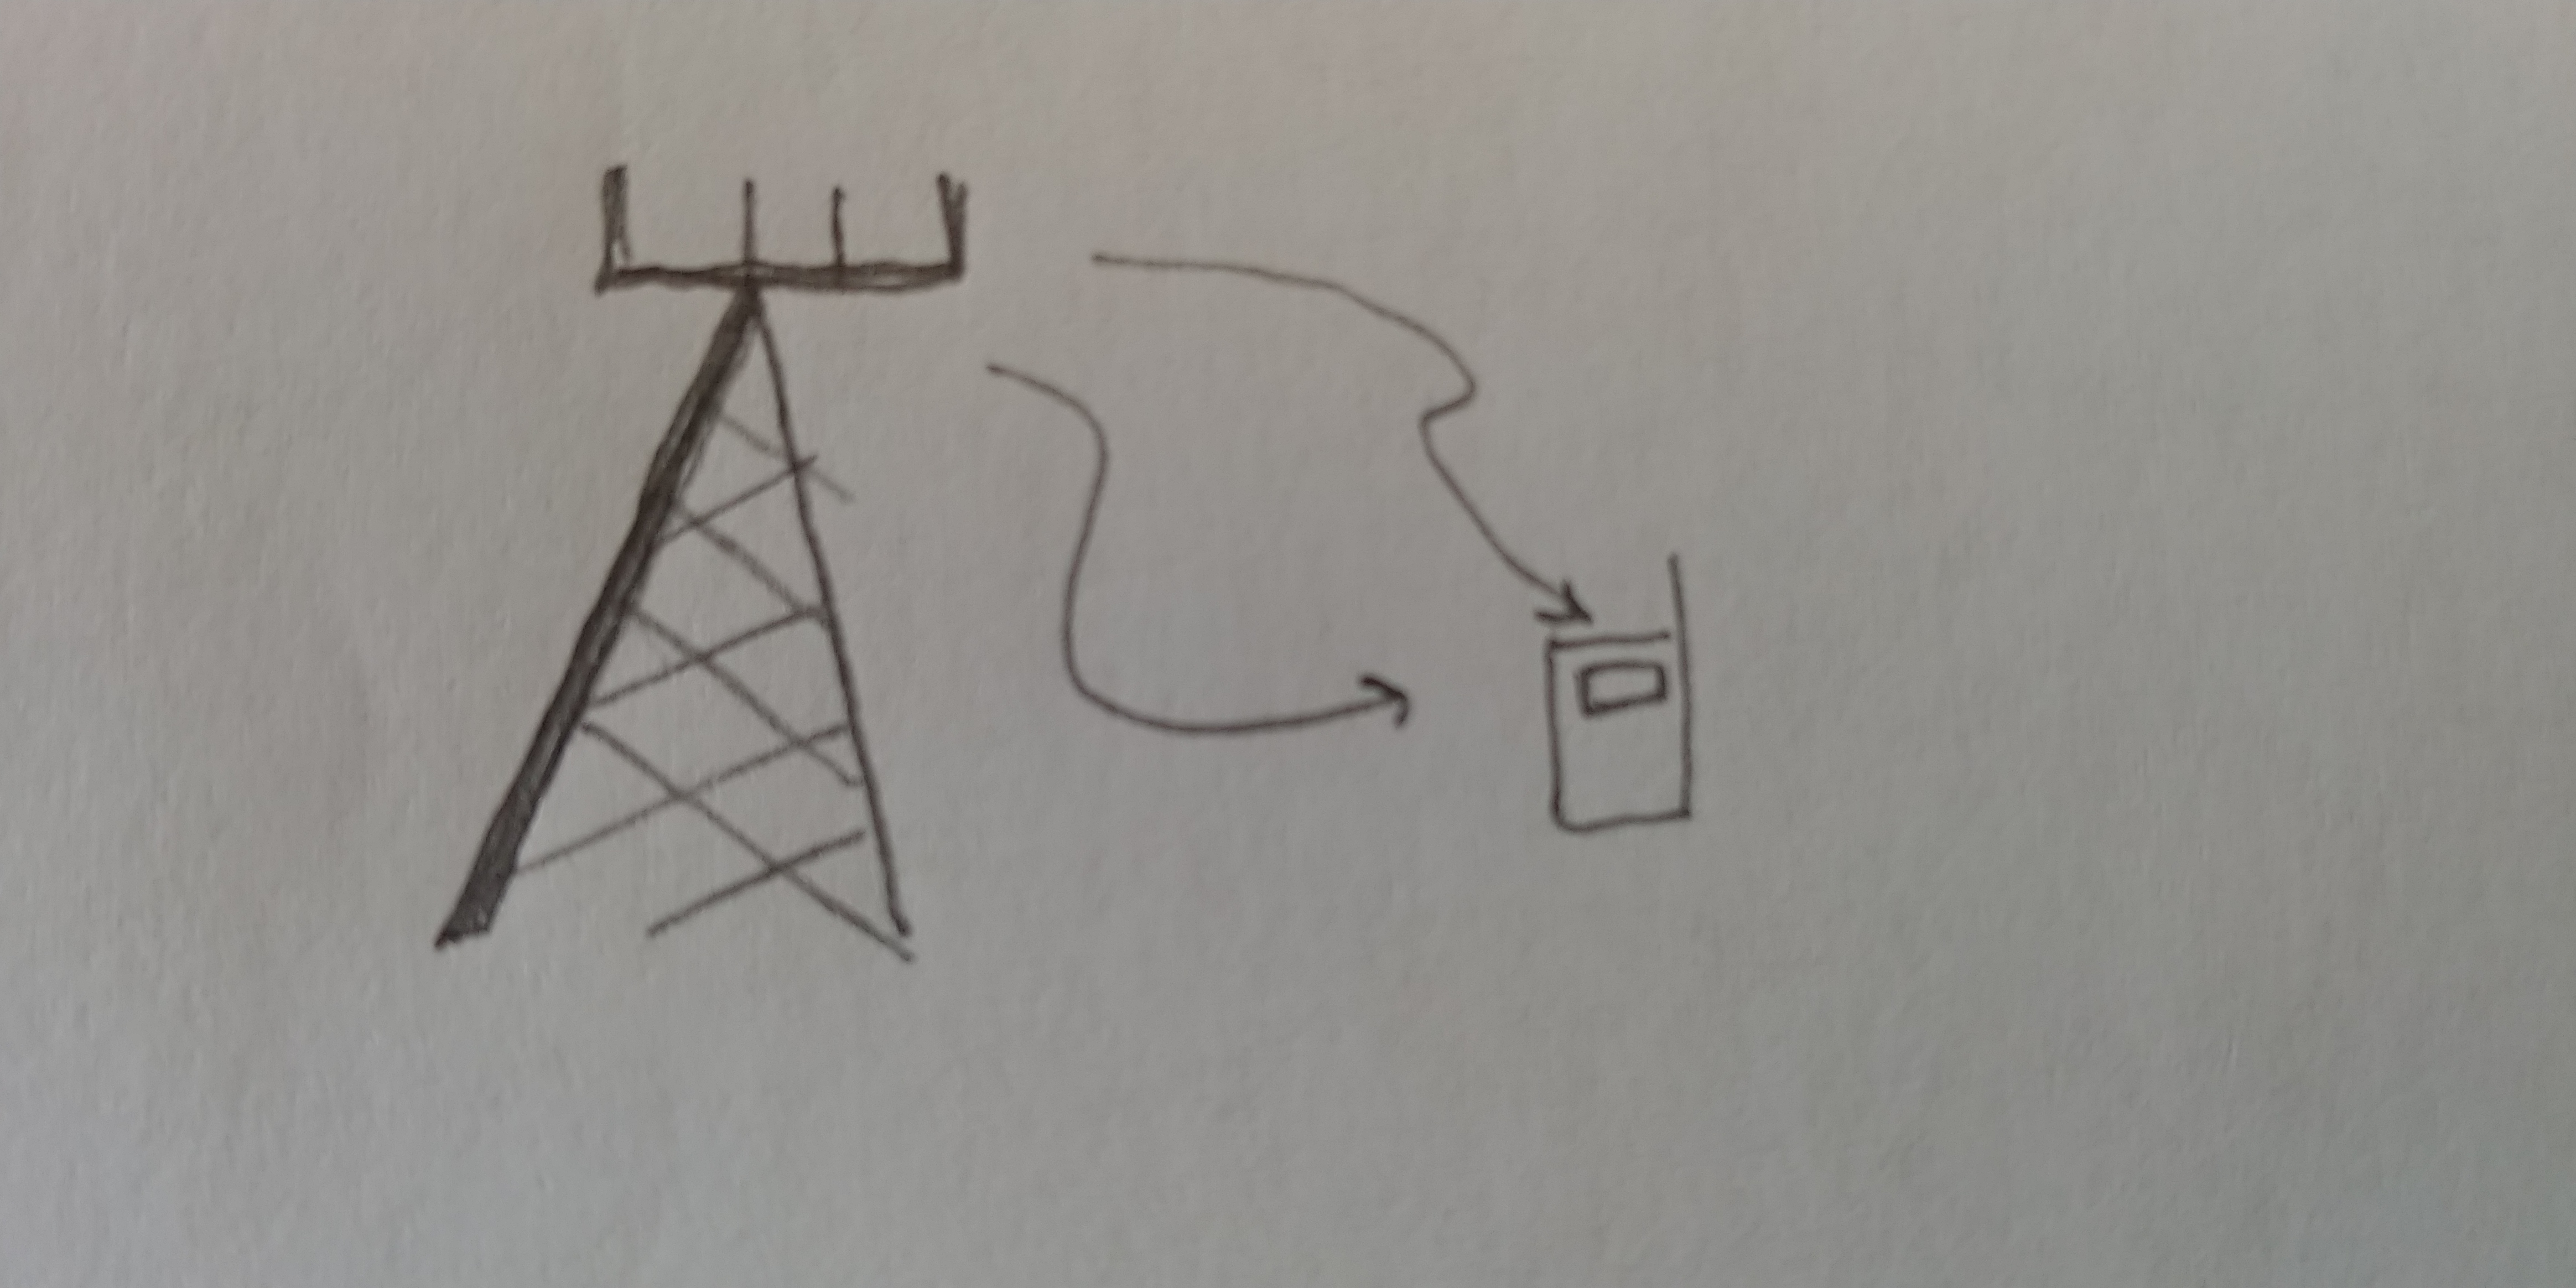
\includegraphics[width=2in]{img/diversi_cammini.jpg}
    \centering
    \caption{Diversit\'a di cammino}
\end{wrapfigure}
Antenne multiple in trasmissione ed antenna unica in recezione $\rightarrow$ diversit\'a di trasmissione

Usando antenne multiple in recezione, aumenta la velocit\'a di canale esponenzialmente; (Con \textbf{5G} verranno utilizzate almeno 2 antenne per device)


% Desegno 115
Per garantire l'ottimizzazione dell'assegnazione delle assegnazzione delle risorse $\rightarrow$ 3G intrpduce il concetto di ``negoziazione'' delle risorse attraverso \textit{Radio Bearer} $\rightarrow$ Canale di trasporto che consente  di negoziare dati (date bearer) o caratteristiche a livello fisico (Signal bearer)

Gli attributi definiti da questi pacchetti di controllo riguardano:

\begin{enumerate}
    \item throughput
    \item Ritardo trasmissivo
    \item Tasso di errore massimo tollerabile
\end{enumerate}

$\Rightarrow$ Tutto questo porta all'introduzione del concetto di classe  di \textbf{QoS} \textit{Quality of Service}
\begin{samepage}
    \subsection{Classi di QoS di UMTS}
    \textbf{Classi di QoS}:\@\textit{Quality of Service} (conversazionale, streaming, interattiva, background), legato alla pianificazione delle reti (dipende dal numero di utenti per cella). Introdotto nella terza generazione.
    \begin{itemize}
        \item \textbf{Conversazionale}: applicazione principale per voce, videogiochi e videotelefonia;
            \begin{itemize}
                \item deve essere preservata l'interazione temporale tra le informative del flusso
                \item Bassa varianza dei ritardi
                    % Image 2

                    \begin{figure}[h]
                        \centering

                        \begin{tikzpicture}
                            \begin{axis}[
                                unit vector ratio*=1 1 1,
                                xmax=2,
                                xmin=-1,
                                xticklabel=\empty,yticklabel=\empty,
                                axis y line = left,
                                samples=200,
                                axis x line = bottom,
                                width=10cm]
                                \addplot[color=red]
                                    {exp(-((x)^2/0.01))};
                            \end{axis}
                        \end{tikzpicture}

                        \caption{Classe Conversazionale}
                    \end{figure}
                \item \'e sopportabile la perdita di alcuni frame, ma non il ritardo eccessivo dell'arrivo di ogni frame

            \end{itemize}

        \item \textbf{Streaming}: Streaming multimediale
            \begin{itemize}
                \item no vincoli su ritardi
                \item perservazione temporale tra i frame

                    % Image 3
                    \begin{figure}[h]
                        \centering
                            \begin{tikzpicture}
                                \begin{axis}[
                                    unit vector ratio*=1 1 1,
                                    xmax=6,
                                    xticklabel=\empty,yticklabel=\empty,
                                    ymax=3,
                                    axis y line = left,
                                    axis x line = bottom,
                                    width=10cm]
                                    \addplot[color=red]
                                        {exp(-((x)^2)/5)};
                                \end{axis}
                            \end{tikzpicture}
                            \caption{Grafico Streaming}
                        \end{figure}
                \end{itemize}

            \item \textbf{Interattiva}: Cadono i requisiti delle entit\'a informative, siccome non \'e piu presente un flusso di dati
                \begin{itemize}
                    \item ottenere risposta da entit\'a remota
                    \item preservare integrit\'a dei dati
                \end{itemize}

        \item \textbf{Background}: Chiede solo di preservare l'integrit\'a dei dati, (Es: Download delle email in background)

            Hanno la minore priorit\'a rispetto alle altre classi di traffico

    \end{itemize}
\end{samepage}
% Disegno 117
Sistema UMBS \'e di fatto formato da 2 sottoinsiemi (che sono l'evoluzione del BSS e NSS)

\textbf{NSS} $\rightarrow$ \textit{Core Network} (CN) $\rightarrow$ autenticazione utenti connessi, commutazione autenticazione connessione, interconnessione verso reti esterne (di altri provider o internet)

\textbf{BSS} $\rightarrow$ \textit{UMTS} Radio Access Network (\textit{UTRAN})


Nella fase iniziale del $3G$ coesistenza di sistemi di 2\textsuperscript{a} e 3\textsuperscript{a} generazione

Con la 3\textsuperscript{a} generazione si inizia ad affiancare la rete d'accesso con la rete d'accesso \textit{UTRAN}

\textbf{CS}: Circuit switching

\textbf{PS}: Packet Switching

\textbf{RNC}: Radio network Controller $\rightarrow$ novit\'a introdotta dalla 3G, Collegati con interfaccia \textbf{Iur}, idealmente sono tutti connessi tra loro

Idea del 3G:\@ Delegare all'esterno pi\'u responsabilit\'a ed intelligenza, mentre lascia all'interno della core Network la tariffazione

%Disegno 118

\textbf{UTRAN} $\rightarrow$ formata da vari RNS, ogniuno dei quali \'e formato da diversi Node B. Ogni Node B gestisce un certo numero di \notate{\text{celle (da 3 a 6)}}{1}{\text{In ogni cella \'e supportato FDD e TDD}}

\begin{samepage}
\subsection{Architettura UTRAN}
\textit{UMTS Terrestrial Radio Area Network}

\begin{figure}[h]
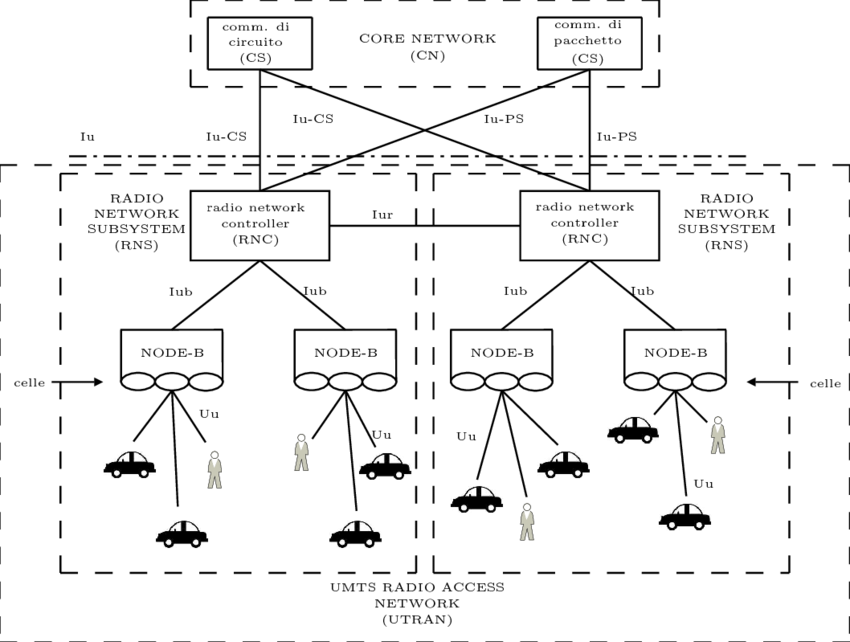
\includegraphics[width=0.8\textwidth]{img/sdt/architettura_utran}
\centering
\end{figure}


Con UTRAN si indica l'insieme dei Node-B e dei Radio Network Controller (RNC), che formano la rete d'accesso radio nello standard UMTS. Contiene:

\begin{itemize}
    \item Interfaccia \textbf{Iu}: Connette RNC alla Core Network (CN). Pi\'u nello specifico viene detta:
        \begin{itemize}
            \item \textbf{Iu-CS} (Circuit Switching) per traffico vocale (connessione con dominuo a circuito)
            \item \textbf{Iu-PS} (Packet Swtiching)  per traffico dati (connessione con dominio a pacchetto)
        \end{itemize}

    \item Interfaccia \textbf{Uu}: Interfaccia telefono e Node B, ha il compito di
        \begin{itemize}
            \item trasportare i servizi per l'utente
            \item Gestione della mobilit\'a: Trasporto delle informazioni necessarie
        \end{itemize}

    \item Interfaccia \textbf{Iub}: Interfaccia di collegamento fra Node B ed il proprio RNC
    \item Interfaccia \textbf{Iur}: Collega RNC appeartenenti a diversi RNS
\end{itemize}


\end{samepage}

La novit\'a a livello architetturale dell'UMTS \'e la presenza degli RNC nella UTRAN . Ogni RNC gestisce tutte le funzionalit\'a lato utente (Mobilit\'a e Assegnazione risorse) senza il bisogno di fare richieste alla Core Network.

Compito del \textbf{Node B}:
\begin{itemize}
    \item Realizzare le trasmissioni radio (modulazione, potenza trasmissiva, gestire il controllo di potenza)
    \item Riceve dal proprio RNC le indicazioni sulle risore da assegnare agli utenti
    \item Effettuare misure sulla potenza e QoS
\end{itemize}


% Drift and Serving RNC
% Lezione 21 - 5 -19
\section{LTE (4G)}
\textit{Long Term Evolution}

Vuole promuovere l'utilizzzo della \textit{banda larga} in mobilit\'a, con l'obbiettivo di raggiungere velocit\'a di connessioni wireless superiori anche ad 1Gbit/s.

Machine to machine legata ad IOT (dovrebbe rimanere piccola siccome i dati trasmessi sono pochi)

Con LTE il traffico vocale inizia ad essere deflesso sul traffico dati (Whatsapp, Skype etc.)

Parte integrante dell'UMTS, ma prevede numerose modifiche:
\begin{itemize}
    \item Resource Scheduling in Uplink e Downlinkm

        Utilizza OFDM (\textit{Orthogonal Frequency Division Multiplexing}) per il downlink e Single-Carrier FDMA per l'uplink (al posto del W-CDMA)
    \item Ha un efficenza spettrale 3 volte superiore alla versione precedente
    \item Trasport layer tutto orientato ad IP, fondamentale per rendere possibile assegnazione dinamica delle risorse
\end{itemize}

\subsection{LTE performance requirements}
\begin{itemize}
    \item Data rate con picchi di 100 Mb/s, massima banda assegnabile ad un utente $20MHz$

        Dalla terza generazione ci si \'e accorti che il traffico \'e asimmetrico, downlink \'e molto pi\'u utilizzato rispetto all' uplink, per questo motivo, l'efficenza spettrale dell'uplink \'e dimezzata rispetto a quella del downlink

    \item Cell range ideale di qualche Km, idealmente si puntava ad avere celle di 30/100 Km di raggio

    \item Cell Capacity fino a 200 utenti attivi per cella
    \item Mobilit\'a (Sistema ottimizzato per basse mobilit\'a)
    \item Latency
        \begin{itemize}
            \item User Plane (nell'ordine di pochi millisecondi $\approx 5ms$), essenziale per AR \& VR
            \item Control Plane
        \end{itemize}

    \item Improved Spectral efficiency
    \item Broadcasting: Tutte le applicazioni legate al Digital Video Broadcasting, (es Eventi in diretta)
    \item Ottimizzato verso l'IP, per essere direttamente compatibili con Internet
    \item Bande scalabili (Attraverso \textbf{OFDMA} consente assegnazioni flessibili di risorse frequenziali)
    \item Co-esistenza con precedenti versioni delle reti cellulari
\end{itemize}

\subsection{3 principali limitazioni del 3G}
\begin{enumerate}
    \item Massima bit rate  % perso
    \item 3\textsuperscript{a} gen non era stata progettata per tenere conto dei vincoli sulla latenza,

        diventa difficile utilizzare applicazioni interattive

        Interazioni ancora peggiori con il resource assignment
    \item 3G richiedeva dei terminali complessi, per funzionare bene c'era bisogno utilizzare dei ricevitori RAKE (molto complessi), i quali richiedevano un grande consumo di batteria
\end{enumerate}

Latenza $\coloneqq$ Round trip delay

\subsection{LTE Architecture}
\textit{High Speed OFDM Packet Access}/\textit{Evolved UTRAN}, due termini per indicare la stessa cosa.
% image 1
\begin{figure}[h]
    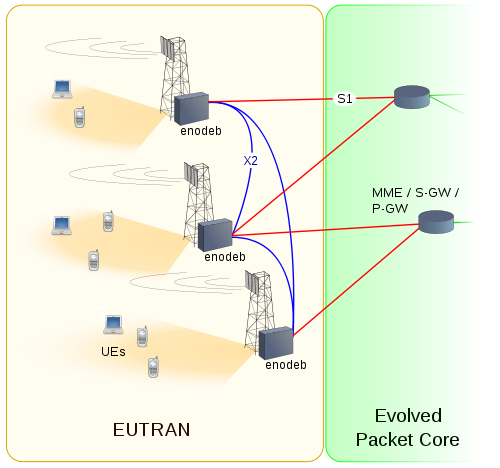
\includegraphics[width=0.5\textwidth]{img/sdt/eutran}
    \centering
    \caption{Architettura E-UTRAN}
    \label{fig:lte_architecture}
\end{figure}

%SAE $\coloneqq$ System Artchitecture Evolution

\textbf{enodeB}: Evolved Node B, parlano direttamente con un Gateway (MME), prende il posto del nodeB ed RNC. L'obbiettivo \'e semplificare la struttura, riducendo la latenza e ridurre l'esposizione all'interferenza radio.
enodeB Contiene uno scheduler che assegna le risorse a tutti gli utenti connessi.

Delegando le capacit\'a gestionali all'enodeB il sistema diventa pi\'u semplice e reattivo.
Ruoi delegati all'eNB
\begin{itemize}
    \item Resource Scheduling
    \item QoS Aware
    \item Autoconfigurarsi rispetto alla posizione nella rete
\end{itemize}

Esistono due tipologie di Gateway

La \textit{Core Network} del 3GPP LTE, si chiama SAE (\textit{System Architecture Evolution}).
\'E la diretta evoluzione della core network utilizzata nel GPRS, ma pi\'u semplificata, ed ha un maggiore thrughput ed una minore latenza.

\subsubsection{EPC}
\textit{Evolved Packet Core}, composto da:
\begin{figure}[h]
    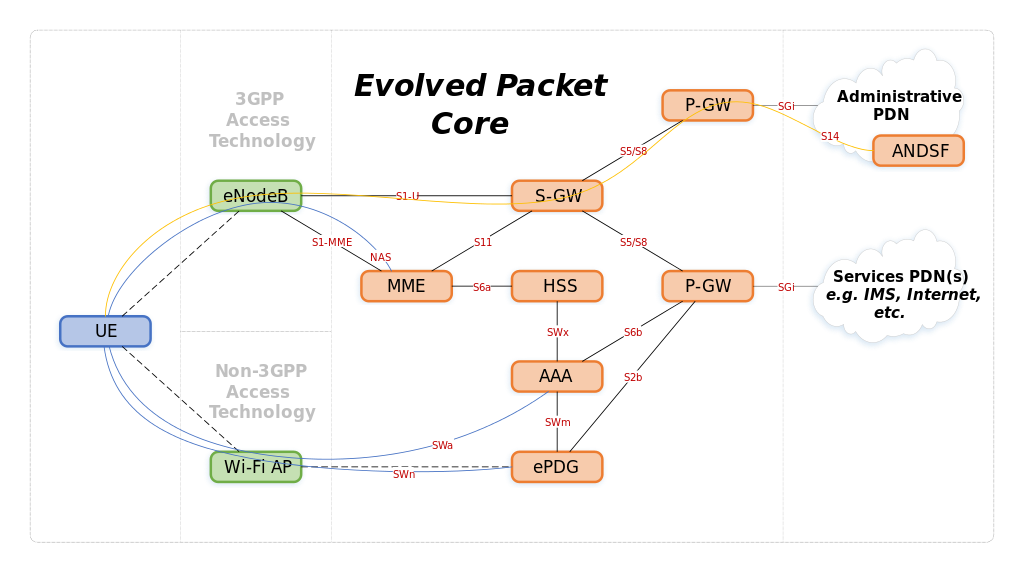
\includegraphics[width=0.8\textwidth]{img/sdt/Evolved_Packet_Core}
    \centering
\end{figure}

\begin{itemize}
    \item MME (\textit{Mobility Management Entity}): Responsabile della gestione utenti (Autenticazione attraverso HSS, Ritrasmissione dati, Generazione Identit\'a temporanee)

        HARQ (\textit{Hybrid Automatic Repeat Request}, H/H+): Algoritmo di error detection, Cerca di accelerare il pi\'u possibile la trasmissione, non interrompendo il flusso

        PCRF (\textit{Policy and Changing Rules Function}): Software che si occupa della tariffazione
    \item HSS (\textit{Home Subscriber Server}, database centrale. Basato sul HLR ed AuC (\textit{Authentication Center}).

        Sostituisce HLR e VLR

\end{itemize}


Architettura semplice dal punto di vista dell'user plane: 3 passi raggiongere l'esterno

Da punto di vista dell'accesso, si concentra tutto sugli eNB


\begin{itemize}
    \item Scompare completamente il CS domain, viene tutto orientato al Packet Switching

    \item  Prepared for Non-3GPP Access

        ePC deve essere in grado di gestire flussi informativi non necessariamente legati a rete cellulare,
        ma anche da access point WiFi
\end{itemize}

% \textbf{IETF}: Internet Engeneering Task Force, si occupa di standardizzare qualsiasi protocollo legato ad internet,
% fondamentalmente libera, per proporre qualcosa di nuovo vengono richiesti degli RFC (Request For Comments)
%
% Si occupano di sviluppare i protocolli, non di come vengono trasmessi i dati


In Uplink, anche se ogniuno ha una singola antenna, nel caso di Cooperazione viene creata una \textit{Antenna Array} $\rightarrow$ Multiuser Collaborative MIMO (Mai implementata)

Uplink max: $75Mbps$

%Appunti Mon 27 May 2019 10:23:18 AM CEST

\section{OFDM}
\textit{Orthogonal Frequency Division Multiplexing}, tecnica di trasmissione che consesnte un tipo di modulazione a multi-portante, i.e. utilizza un numero elevato di sottoportanti tra loro ortogonali.

\begin{figure}[h]
    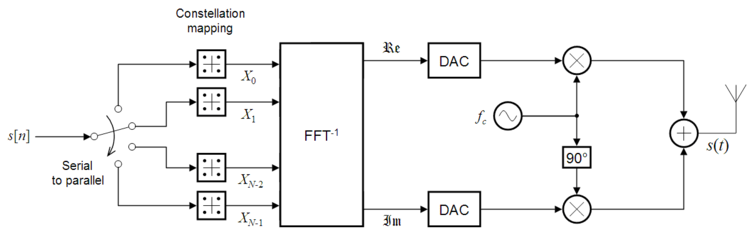
\includegraphics[width=0.8\textwidth]{img/sdt/ofdm_transmitter}
    \centering
    \caption{Trasmettitore OFDM}
\end{figure}

Ogni portante \'e modulata attraverso una modulazione di tipo convenzionale (es. QPSK) con basso symbol rate.

Il vantaggio primario dell'OFDM rispetto agli schemi a singola portante \'e l'abilit\'a di comunicare anche in condizioni pessime di canale. Mantenere un basso symbol rate permette di rudurre l'interferenza intersimbolica grazie ad intervalli di guardia. Fintanto che tutti i segnali e le loro repliche da cammino multiplo rientrano  nel periodo di guardia, non c\'e interferenza intersimbolo.

La trasmissione viene divisa in N flussi paralleli, poi fatta passare per un codificatore di costallazione ed un modulatore elementare.
Tutti gli N flussi vengono creati allo stesso istante, poi passati ai modulatori, che possono modulare il segnale in sottoportanti equamente distanziate tra loro (Per l'LTE questa distanza \'e $\approx$ 15KHz).

Le sottoportanti sono scelte in modo da essere ortogonali tra loro, riducendo cosi la mutua inteferenza.
Ortogonalit\'a significa anche un elefata efficienza spettrale, a parit\'a di BitRate.

La codifica del segnale \'e basata sull'FFT inversa, (a recezione per riottenere il segnale baster\'a riapplicare FFT).

La suddivisione ortogonale delle frequenze richiede un precisa sincronizzazione tra trasmettitore e ricevitore, richiede quindi un aumento di complessit\'a nel ricevitore.

Un modo per ridurre l'\textbf{interferenza inter simbolo} \'e l'utilizzo trasmettere nel periodo di guardia la parte iniziale o finale del simbolo successivo (CP \textit{Cycling Prefix}) o precedente (CS \textit{Cycling Suffix}).
\subsection{Pulse shaping and spectrum}
Slide 293

% TODO
% https://en.wikipedia.org/wiki/Pulse_shaping
% https://en.wikipedia.org/wiki/Intersymbol_interference
% -Missing-

Il filrtro pi\'u facile da utilizzare \'e l'impulso rettangolare (sync)

Da slide 294: Una serie di impulsi, ricevuti in maniera diversa con diversi ritardi.

A livello temporale si riceve la somma dei segnali ritardati, i quali possono interferire tra di loro (Interferenza da commino multiplo)

Ricevitori \textbf{RAKE} Sfruttano l'evanescenza da cammini multipli per potenziare il segnale

$1^a$ soluzione intuitiva (296): Aggiungere un periodo di guardia (GP): Ritardo tra trasmissione dei simboli
Risolve solo interferenza intersimbolica, non danneggia simboli successivi

L'elaborazione dei segnali diventa molto pi\'u semplice, ma \'e lento, siccome il periodo di Guardia \'e tempo non utilizzato $\rightarrow$ Non efficente

Un altro problema lo si ha se si manifestano ritardi pi\'u alti del periodo di guardia


Supponendo di utilizzare comunque questo approccio, per proteggersi dalle interferenze residue: Una delle repliche ricevute \'e piu forte delle altre. Supponendo che l'interferenza avvenga solamente all'inizio del simbolo: Prefisso e Suffisso ciclico (298)

Prefisso ciclico: Prendere l'ultima parte del simbolo e la mette all'inizio

Suffisso ciclico: Lo stesso solo che prende la prima parte e la mette alla fine del simbolo

\textbf{Limitazione modulazione a singola portante}
La percentuale del tempo in cui viene trasmesso un simbolo di dati
\[ E = \frac{T_{SYMBOL}}{T_{SYMBOL} + T_{CP}} \]

\subsection{Multi Carrier Modulation}

Generalizzazione FDMA

Esistono ancora le sottobande, ma vengono assegnate tutte ad un unico utente, su ogni sottobanda viene trasmesso un segnale

Per evitare di perdere risorse, si cercano di fare le sottobande pi\'u vicine possibili, ma se sono troppo vicine si rischia l'interferenza da portanti adiacenti

\subsection{OFDM}
Impulso utilizzato: Rettangolare

Densit\'a spettrale in potenza $\propto$ al quadrato della sinc

Idea OFDM: Impacchettare densit\'e spettrali di potenza mantenendo ortogonalit\'a e sfruttando gli zeri delle sinc (305)


\subsection{OFDM ad accesso multiplo}
\textbf{Sistemi multiportante}
% slide 282
Con CDMA veniva assegnata tutta la banda e si sperava che i notch fossero pochi rispetto alla grandezza di banda,

$\Rightarrow$ approccio pi\'u efficente, dividere banda in pi\'u bande piccole ed assegnarne un diverso numero ad un unico utente:
Vengono assegnate solo quelle dove il canale ha una `buon' risposta, in modo da utilizzare al massimo possibile ogni porzinoe di banda


Ogni risorsa frequenziale prende il nome di \textbf{Resource Block}, e corrsiponde ad una sottobanda di $180KHz$.
Vengono assegnati tra i 6 ed i 100 blocchi di risorse in base al tipo di richiesta

Protocolli di accesso multiplo e modelli di scheduling sono identici,

\textbf{OFDMA} legato all'OFDM, Include anche il livello fisico

Diversi approcci:
\begin{enumerate}
    \item slide 309 (Un unico trasmettitore)
    \item TDMA (Trasmettitori multipli)

        Limitato:
        Se solo uno deve trasmettere, molte risorse rimangono inutilizzzate

        Introdotto il concetto di blocco di risorse:
        Posso assegnare le risorse in modo diverso in base alle esigenze deglu utenti (Slide 311)

        12 sottoportanti formano un blocco di risorse

\end{enumerate}
Le sottoportanti vengono assegnate in base alla risposta dei vari utenti sul canale di comunicazione

(slide 319):
Superficie gialla presa in un istante temporale (proiezione su asse z-frequenza): Come cambia la risposta in frequenza del canale all'avanzare del tempo, cambia in modo regolare

Blu: per un altro utente (non sono uguali giallo-blu)

La base station ad un certo istante guarda le risposte in frequenza ed in base ad esse sceglie a quale utente assegnare le sottofrequenze

(Scheduling utilizzato nei sistemi di $4^a$ generazione, tipicamente funzionano in modalit\'a TDD, (Trasmissioni suddivise in Uplink e Downlink). Tra le due fasi c\'e una fase di negoziazione, dove vengono riassegnate le risorse per il successivo Uplink/Downlink

Utilizza efficentemente le risorse del canale

LTE utilizza OFDMA in Downlink; Per l'Uplink SC-FDMA

\textbf{SC-FDMA Single Carrier Frequency Division Multiple Access}

Funziona molto bene per valori relativamente bassi di PAPR

PAPR: Peack to Average Power Ratio (Rapporto di potenza fra picco e media), Caratterizza la qualit\'a del segnale trasmesso

(Slide 318) Come Viene implementato l'OFDMA nell'LTE

$5G$ Inizier\'a a funzionare utilizzando l'OFDMA come formato di modulazione

(323) Durada di uno slot in base alla grandezza del prefisso ciclico

LTE modalit\'a FDD (325)

LTE modalit\'a TDD (326)
Configurazione
\begin{itemize}
    \item Downlink
    \item Sincronizzazione
    \item Uplink
    \item Uplink
    \item Uplink
    \item Downlink
    \item Sincronizzazione
    \item Uplink
    \item Uplink
    \item Uplink
\end{itemize}

In basso a sinistra (sempre 326) Configurazioni personali per ogni utenti, assegnate automaticamente tenendo conto dello stato dell'utente

In un blocco di risorse non \'e detto che venga utilizzato lo stesso formato di modulazione

% Lezione 13/05/19 (di vodafone)
\section{5G}

\subsection{Advanteges over 4G}

\begin{itemize}
    \item Maggiore disponibilit\'a di banda
    \item Bassa latenza: da 9 a 10 ms; Dovuta alla minore distanza cloud-server\\
        Multiaccess Edge Computing: Place more computing resource closer to the point of data creation\\
        Very useful for AR/VR

    \item Maggior numero di dispositivi connessi per km\textsuperscript{2} (1 mln)
    \item Peak data rate from 1\(Gbs\) to 20\(Gbs\)
    \item Available spectrum from 3\(GHz\) to 30\(GHz\)
    \item Higher data traffic; from 7.2 Exabyte/Month to 50 Exabyte/Month

\end{itemize}

Non acora pienamente utilizzato, verr\'a utilizzato maggiormente con \textit{IOT}

5G will become the backbone of Smart Cities, diriverless car… (IOT, Industria 4.0)

\textbf{Sistemi multiportante}
% slide 282
Con CDMA veniva assegnata tutta la banda e si sperava che i notch fossero pochi rispetto alla grandezza di banda,

$\Rightarrow$ approccio pi\'u efficente, dividere banda in pi\'u bande piccole ed assegnarne un diverso numero ad un unico utente:
Vengono assegnate solo quelle dove il canale ha una `buon' risposta, in modo da utilizzare al massimo possibile ogni porzinoe di banda


Ogni risorsa frequenziale prende il nome di \textbf{Resource Block}, e corrsiponde ad una sottobanda di $180KHz$.
Vengono assegnati tra i 6 ed i 100 blocchi di risorse in base al tipo di richiesta

Protocolli di accesso multiplo e modelli di scheduling sono identici,

\textbf{OFDMA} legato all'OFDM, Include anche il livello fisico
\end{document}
